% Options for packages loaded elsewhere
\PassOptionsToPackage{unicode}{hyperref}
\PassOptionsToPackage{hyphens}{url}
%
\documentclass[
]{book}
\title{Analisis Regresi}
\usepackage{etoolbox}
\makeatletter
\providecommand{\subtitle}[1]{% add subtitle to \maketitle
  \apptocmd{\@title}{\par {\large #1 \par}}{}{}
}
\makeatother
\subtitle{Sebuah Referensi Singkat dengan Menggunakan R}
\author{Tedy Herlambang}
\date{2022-01-21}

\usepackage{amsmath,amssymb}
\usepackage{lmodern}
\usepackage{iftex}
\ifPDFTeX
  \usepackage[T1]{fontenc}
  \usepackage[utf8]{inputenc}
  \usepackage{textcomp} % provide euro and other symbols
\else % if luatex or xetex
  \usepackage{unicode-math}
  \defaultfontfeatures{Scale=MatchLowercase}
  \defaultfontfeatures[\rmfamily]{Ligatures=TeX,Scale=1}
\fi
% Use upquote if available, for straight quotes in verbatim environments
\IfFileExists{upquote.sty}{\usepackage{upquote}}{}
\IfFileExists{microtype.sty}{% use microtype if available
  \usepackage[]{microtype}
  \UseMicrotypeSet[protrusion]{basicmath} % disable protrusion for tt fonts
}{}
\makeatletter
\@ifundefined{KOMAClassName}{% if non-KOMA class
  \IfFileExists{parskip.sty}{%
    \usepackage{parskip}
  }{% else
    \setlength{\parindent}{0pt}
    \setlength{\parskip}{6pt plus 2pt minus 1pt}}
}{% if KOMA class
  \KOMAoptions{parskip=half}}
\makeatother
\usepackage{xcolor}
\IfFileExists{xurl.sty}{\usepackage{xurl}}{} % add URL line breaks if available
\IfFileExists{bookmark.sty}{\usepackage{bookmark}}{\usepackage{hyperref}}
\hypersetup{
  pdftitle={Analisis Regresi},
  pdfauthor={Tedy Herlambang},
  hidelinks,
  pdfcreator={LaTeX via pandoc}}
\urlstyle{same} % disable monospaced font for URLs
\usepackage{color}
\usepackage{fancyvrb}
\newcommand{\VerbBar}{|}
\newcommand{\VERB}{\Verb[commandchars=\\\{\}]}
\DefineVerbatimEnvironment{Highlighting}{Verbatim}{commandchars=\\\{\}}
% Add ',fontsize=\small' for more characters per line
\usepackage{framed}
\definecolor{shadecolor}{RGB}{248,248,248}
\newenvironment{Shaded}{\begin{snugshade}}{\end{snugshade}}
\newcommand{\AlertTok}[1]{\textcolor[rgb]{0.94,0.16,0.16}{#1}}
\newcommand{\AnnotationTok}[1]{\textcolor[rgb]{0.56,0.35,0.01}{\textbf{\textit{#1}}}}
\newcommand{\AttributeTok}[1]{\textcolor[rgb]{0.77,0.63,0.00}{#1}}
\newcommand{\BaseNTok}[1]{\textcolor[rgb]{0.00,0.00,0.81}{#1}}
\newcommand{\BuiltInTok}[1]{#1}
\newcommand{\CharTok}[1]{\textcolor[rgb]{0.31,0.60,0.02}{#1}}
\newcommand{\CommentTok}[1]{\textcolor[rgb]{0.56,0.35,0.01}{\textit{#1}}}
\newcommand{\CommentVarTok}[1]{\textcolor[rgb]{0.56,0.35,0.01}{\textbf{\textit{#1}}}}
\newcommand{\ConstantTok}[1]{\textcolor[rgb]{0.00,0.00,0.00}{#1}}
\newcommand{\ControlFlowTok}[1]{\textcolor[rgb]{0.13,0.29,0.53}{\textbf{#1}}}
\newcommand{\DataTypeTok}[1]{\textcolor[rgb]{0.13,0.29,0.53}{#1}}
\newcommand{\DecValTok}[1]{\textcolor[rgb]{0.00,0.00,0.81}{#1}}
\newcommand{\DocumentationTok}[1]{\textcolor[rgb]{0.56,0.35,0.01}{\textbf{\textit{#1}}}}
\newcommand{\ErrorTok}[1]{\textcolor[rgb]{0.64,0.00,0.00}{\textbf{#1}}}
\newcommand{\ExtensionTok}[1]{#1}
\newcommand{\FloatTok}[1]{\textcolor[rgb]{0.00,0.00,0.81}{#1}}
\newcommand{\FunctionTok}[1]{\textcolor[rgb]{0.00,0.00,0.00}{#1}}
\newcommand{\ImportTok}[1]{#1}
\newcommand{\InformationTok}[1]{\textcolor[rgb]{0.56,0.35,0.01}{\textbf{\textit{#1}}}}
\newcommand{\KeywordTok}[1]{\textcolor[rgb]{0.13,0.29,0.53}{\textbf{#1}}}
\newcommand{\NormalTok}[1]{#1}
\newcommand{\OperatorTok}[1]{\textcolor[rgb]{0.81,0.36,0.00}{\textbf{#1}}}
\newcommand{\OtherTok}[1]{\textcolor[rgb]{0.56,0.35,0.01}{#1}}
\newcommand{\PreprocessorTok}[1]{\textcolor[rgb]{0.56,0.35,0.01}{\textit{#1}}}
\newcommand{\RegionMarkerTok}[1]{#1}
\newcommand{\SpecialCharTok}[1]{\textcolor[rgb]{0.00,0.00,0.00}{#1}}
\newcommand{\SpecialStringTok}[1]{\textcolor[rgb]{0.31,0.60,0.02}{#1}}
\newcommand{\StringTok}[1]{\textcolor[rgb]{0.31,0.60,0.02}{#1}}
\newcommand{\VariableTok}[1]{\textcolor[rgb]{0.00,0.00,0.00}{#1}}
\newcommand{\VerbatimStringTok}[1]{\textcolor[rgb]{0.31,0.60,0.02}{#1}}
\newcommand{\WarningTok}[1]{\textcolor[rgb]{0.56,0.35,0.01}{\textbf{\textit{#1}}}}
\usepackage{longtable,booktabs,array}
\usepackage{calc} % for calculating minipage widths
% Correct order of tables after \paragraph or \subparagraph
\usepackage{etoolbox}
\makeatletter
\patchcmd\longtable{\par}{\if@noskipsec\mbox{}\fi\par}{}{}
\makeatother
% Allow footnotes in longtable head/foot
\IfFileExists{footnotehyper.sty}{\usepackage{footnotehyper}}{\usepackage{footnote}}
\makesavenoteenv{longtable}
\usepackage{graphicx}
\makeatletter
\def\maxwidth{\ifdim\Gin@nat@width>\linewidth\linewidth\else\Gin@nat@width\fi}
\def\maxheight{\ifdim\Gin@nat@height>\textheight\textheight\else\Gin@nat@height\fi}
\makeatother
% Scale images if necessary, so that they will not overflow the page
% margins by default, and it is still possible to overwrite the defaults
% using explicit options in \includegraphics[width, height, ...]{}
\setkeys{Gin}{width=\maxwidth,height=\maxheight,keepaspectratio}
% Set default figure placement to htbp
\makeatletter
\def\fps@figure{htbp}
\makeatother
\setlength{\emergencystretch}{3em} % prevent overfull lines
\providecommand{\tightlist}{%
  \setlength{\itemsep}{0pt}\setlength{\parskip}{0pt}}
\setcounter{secnumdepth}{5}
\usepackage{booktabs}
\usepackage{amsthm}
\makeatletter
\def\thm@space@setup{%
  \thm@preskip=8pt plus 2pt minus 4pt
  \thm@postskip=\thm@preskip
}
\makeatother
\ifLuaTeX
  \usepackage{selnolig}  % disable illegal ligatures
\fi
\usepackage[]{natbib}
\bibliographystyle{apalike}

\begin{document}
\maketitle

{
\setcounter{tocdepth}{1}
\tableofcontents
}
\begin{center}\rule{0.5\linewidth}{0.5pt}\end{center}

Analisis Regresi: Sebuah Referensi Singkat dengan Menggunakan R \textbar{} Analisis Regresi

\hypertarget{analisis-regresi-sebuah-referensi-singkat-dengan-menggunakan-r}{%
\chapter*{Analisis Regresi: Sebuah Referensi Singkat dengan Menggunakan R}\label{analisis-regresi-sebuah-referensi-singkat-dengan-menggunakan-r}}
\addcontentsline{toc}{chapter}{Analisis Regresi: Sebuah Referensi Singkat dengan Menggunakan R}

\hypertarget{tedy-herlambang}{%
\section*{\texorpdfstring{\emph{Tedy Herlambang}}{Tedy Herlambang}}\label{tedy-herlambang}}
\addcontentsline{toc}{section}{\emph{Tedy Herlambang}}

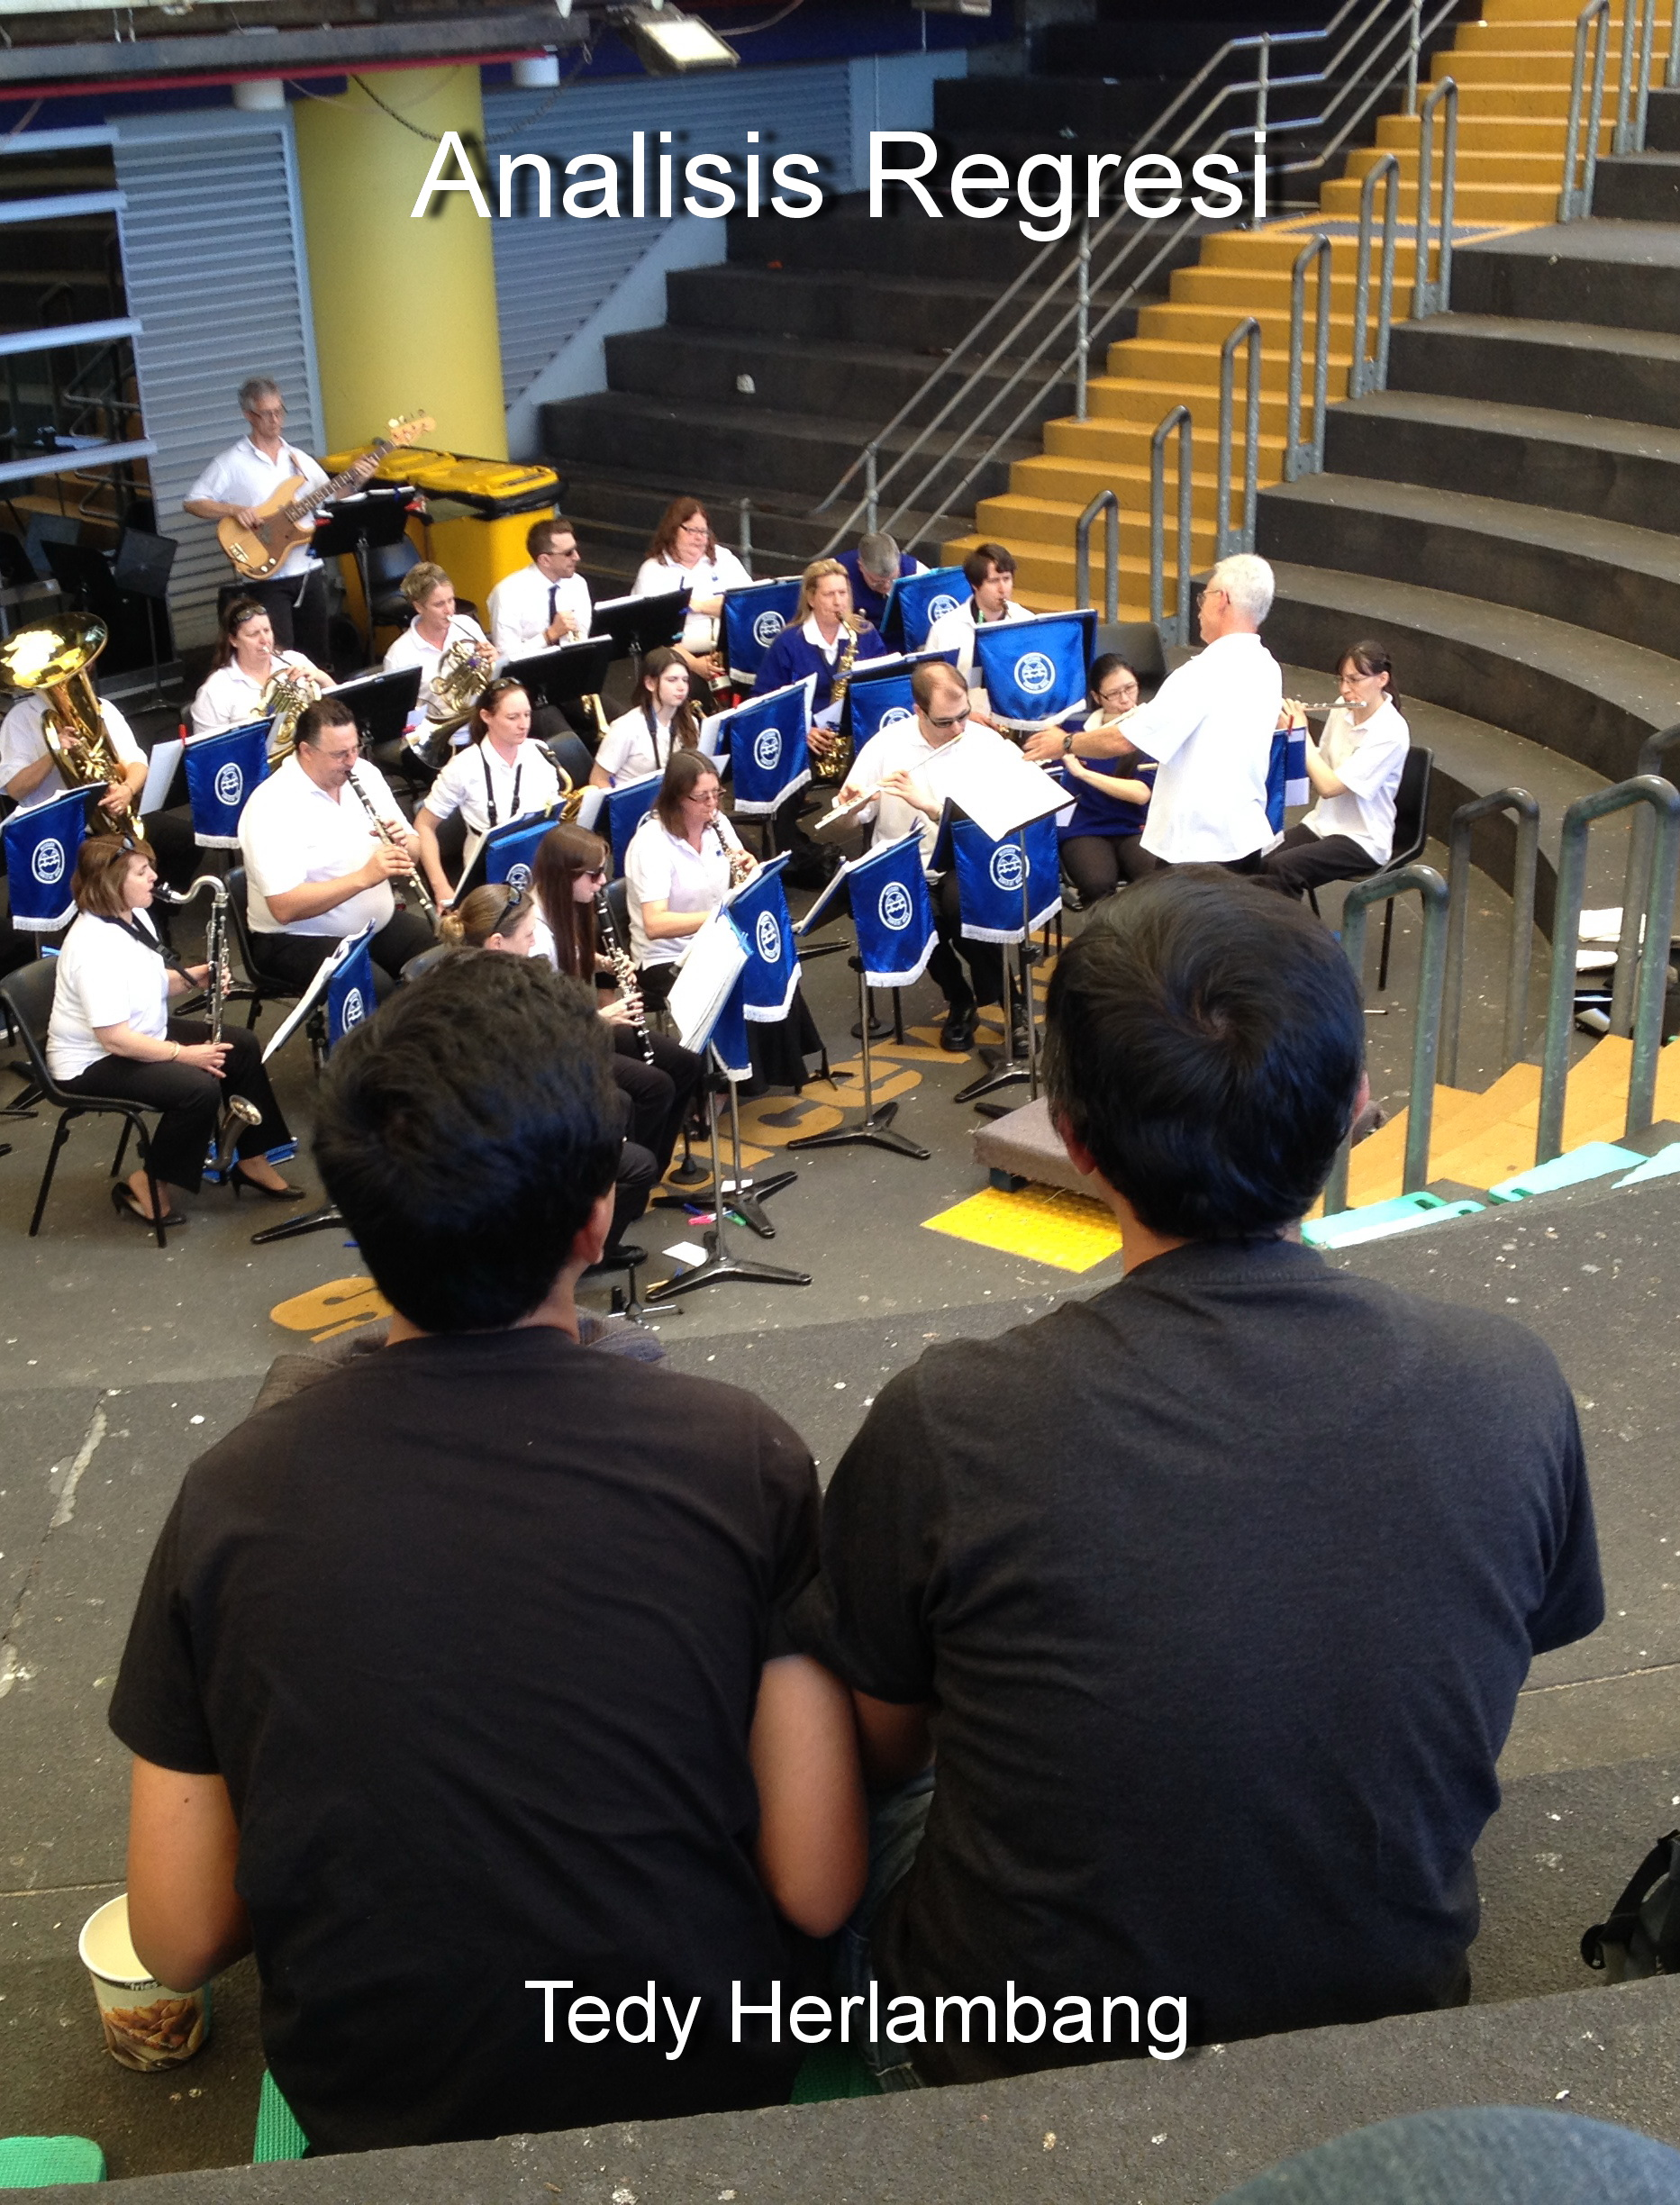
\includegraphics[width=3.38542in,height=\textheight]{images/analisisregresi.jpg}

\hypertarget{kata-pengantar}{%
\chapter*{Kata Pengantar}\label{kata-pengantar}}
\addcontentsline{toc}{chapter}{Kata Pengantar}

Manusia sering menghubung-hubungkan suatu hal dengan hal yang lain. Sebaiknya kita menyimpulkan hubungan ini atas dasar bukti-bukti sahih, bukan spekulasi. Salah satu alat yang bisa dipakai untuk membuktikan adanya hubungan antar variabel adalah analisis regresi.

Analisis regresi mengekplorasi hubungan antara satu variabel, biasa disebut sebagai variabel respons dengan satu atau lebih variabel prediktor/penjelas kemudian mengekspresikan hubungan ini dalam sebuah fungsi. Pengetahuan dan ekspresi hubungan ini dapat dipakai untuk membuat prediksi dan mengidentifikasi variabel-variabel yang paling berpengaruh terhadap sebuah variabel respons. Sebagai misal kita memprediksi keberhasilan studi dan prestasi kerja seseorang (respons) berdasarkan IQ, jenis kelamin, latar belakang sosial-ekonomi dan pendidikan ortunya (prediktor). Prediksi menguji kemampuan kita memetakan variabel-variabel yang paling berpengaruh terhadap suatu variabel respons. Jika kita tidak tepat mengidentifikasi variabel-variabel ini, prediksi dan skenario yang kita buat bisa meleset.

Analisis regresi mencakup metode grafik dan analitik. Dengan bantuan komputer dan pemikiran yang cermat, analisis regresi dapat menjadi alat untuk membedah data yang kompleks menjadi informasi yang berguna. Tetapi, komputer tidak bisa berpikir dan merencanakan sendiri. Komputer hanya membantu kita melakukan perhitungan dengan cepat, agar kita memiliki lebih banyak waktu untuk berpikir dan memperbaiki model analisis.

Di dalam buku singkat ini, saya akan membahas analisis regresi dan penerapannya. Pembahasan dimulai dengan regresi linier sederhana, dilanjutkan ke regresi berganda, permasalahan yang biasa kita temui dalam analisis regresi serta analisis regresi lanjutan dan ditutup dengan diskusi. Program yang akan digunakan adalah R \citep{rcoreteam2021} yang bisa diunduh secara gratis di \href{https://www.r-project.org/}{sini}.

Tetapi buku ini bukan buku tentang R. Juga bukan buku tentang statistik. Materi untuk belajar R sangat banyak tersedia secara \emph{online} misalnya \href{https://cran.r-project.org/doc/manuals/r-devel/R-intro.html}{Introduction to R}. Pembaca juga bisa mengikuti berbagai topik di \href{https://www.r-bloggers.com/}{R-bloggers}. Tujuan buku ini adalah sebagai referensi untuk memperkuat pemahaman pembaca tentang model regresi sebagai salah satu alat analisis yang bisa diterapkan pada berbagai bidang akademik maupun praktik. Saya mengharapkan buku ini bisa menjadi \emph{live book} yang berkembang sesuai saran pembaca. Buku ini adalah versi \emph{online} dari versi cetak yang akan diterbitkan kemudian.

\hypertarget{anda-punya-ide}{%
\section*{Anda punya ide? 📩}\label{anda-punya-ide}}
\addcontentsline{toc}{section}{Anda punya ide? 📩}

Jika Anda punya ide atau topik untuk perbaikan buku ini, atau punya saran dan pengalaman dalam menerapkan konsep-konsep di dalam buku ini, silakan menyampaikan saran Anda ke email: bangtedy (at) gmail.com.

\begin{itemize}
\tightlist
\item
  \href{https://twitter.com/t_hlb}{Twitter}
\item
  \href{https://github.com/bangtedy}{Github}
\end{itemize}

\textbf{Catatan}: \emph{Analisis Regresi: Sebuah Referensi Singkat dengan Menggunakan R}. Hak cipta ada pada Tedy Herlambang dan diedarkan berdasarkan Creative Commons BY-NC-ND 4.0 International License. Anda bebas menggunakan isi buku ini untuk tujuan non-komersial, dengan menyebutkan sumbernya ke https://bangtedy.github.io/analisisregresi.

\emph{Cara mengutip}:

\begin{quote}
Herlambang, Tedy. 2022. Analisis Regresi. URL \url{https://bangtedy.github.io/analisisregresi}.
\end{quote}

\hypertarget{disclaimer}{%
\subsubsection*{Disclaimer}\label{disclaimer}}
\addcontentsline{toc}{subsubsection}{Disclaimer}

The information is this book is provided without warranty. The authors and publisher have neither liability nor responsibility to any person or entity related to any loss or damages arising from the information contained in this book.

\emph{Terakhir diperbarui pada: 21 January 2022}.

\hypertarget{pendahuluan}{%
\chapter{Pendahuluan}\label{pendahuluan}}

Sebagai praktisi atau akademisi, terkadang kita tertarik untuk
meningkatkan pemahaman atas sesuatu dengan menginvestigasinya. Tertulis
atau hanya tercatat di dalam pikiran, di dalam proses investigasi ini,
kita menyusun hipotesis-hipotesis yang ingin kita buktikan kebenarannya.

Untuk sampai pada kesimpulan menolak atau menerima hipotesis-hipotesis
ini, kita merancang investigasinya, mengumpulkan data/bukti-bukti
kemudian menganalisisnya. Di dalam proses analisis ini, seorang investigator biasanya memiliki data sampel yang berasal dari suatu populasi. Hasil analisisnya dapat menyediakan bukti-bukti statistik yang mendukung atau menolak hipotesis yang telah dibuat serta menampilkan karakteristik-karakteristik penting dari populasi dimana data yang dianalisis berasal.

Proses investigasi ini biasanya iteratif, tidak sekali luncur langsung
selesai. Dalam beberapa hal, investigasi harus kita ulang lagi sampai
didapatkan sebuah model statistik yang memuaskan dengan mempertimbangkan
kepraktisan, biaya dan waktu yang tersedia.

Subjek investigasi atau percobaan kita dapat berupa hal-hal yang berada
di dalam atau di luar diri kita, yang kasatmata atau tidak. Aerobiologi
mempelajari partikel-partikel organik (bakteri, spora jamur, polen,
serangga-serangga kecil) yang terbawa udara secara pasif. Astronomi
mempelajari benda langit dan fenomena-fenomena alam yang terjadi di luar
atmosfer bumi. Ilmu Ekonomi mempelajari kegiatan produksi, alokasi dan
distribusi barang dan jasa. Psikologi mempelajari alam pikiran manusia.
Geologi mempelajari bentuk dan komposisi bumi.

Analisis regresi tidak mempelajari suatu subjek secara langsung tetapi
sebagai alat analisis yang dipakai di sebuah bidang ilmu. Kegunaannya
tidak langsung tetapi melalui bantuan yang diberikan ke bidang ilmu
lain.

Analisis regresi sangat berguna, sebab hampir semua cabang ilmu
pengetahuan harus berhubungan dengan data yang tidak sempurna.
Ketidaksempurnaan data ini mungkin terjadi karena kita hanya dapat
mengamati dan mencatat sebagian saja dari apa yang relevan dengan subjek
penelitian kita.

Atau bisa juga karena kita hanya dapat mengamati secara tidak langsung
dari apa yang benar-benar relevan dengan subjek yang diamati. Mungkin
juga karena seberapapun hati-hati kita melakukan observasi atau
mendesain sebuah percobaan, data yang diperoleh akan selalu mengandung
unsur `gangguan' (\emph{noise}).

Analisis regresi adalah salah satu teknik statistik yang paling luas dipakai \citep{agresti2015}; \citep{frees2010} dan \citep{lee2013}.
Penerapannya meliputi hampir semua bidang ilmu: bisnis, ekonomi, teknik,
ilmu-ilmu sosial, biologi dan kesehatan. Pada beberapa proyek penelitian
analisis regresi bahkan seringkali menjadi alat analisis utamanya.
Keberhasilan penerapan model regresi linier memerlukan pemahaman baik
akan teori yang mendasarinya maupun persoalan-persoalan praktis yang
sering terjadi di dalam penggunaan alat analisis ini dalam situasi riil.

\hypertarget{model-regresi-linier}{%
\section{Model Regresi Linier}\label{model-regresi-linier}}

Model di dalam analisis regresi merujuk pada ekspresi matematik yang
menjelaskan perilaku-perilaku dari variabel-variabel yang menjadi
perhatian. Model regresi linier atau biasa disebut analisis regresi
\citep{faraway2015b} digunakan untuk menjelaskan atau memodelkan hubungan
antara satu variabel respons \(y\) dengan satu atau lebih variabel
prediktor \(x_1, x_2, ... , x_p\), dimana \(p\) adalah jumlah prediktor.
Secara khusus, analisis regresi adalah upaya untuk menjelaskan
pergerakan sebuah variabel respons dengan merujuk pada pergerakan satu
atau lebih variabel eksplanatori. Jika \(p=1\), modelnya disebut regresi
sederhana. Tetapi jika \(p>1\), disebut regresi berganda.

Dalam analisis regresi, kita dapat menggunakan pengetahuan tentang
hubungan ini untuk memprediksi respons variabel \(y\) melalui variabel
\(x\). Karena hubungan inilah maka \(y\) disebut variabel respons dan \(x\)
disebut variabel prediktor. Rumpun ilmu berbeda kadang menggunakan
istilah yang berbeda untuk menyebut variabel \(x\) dan \(y\), seperti yang ditunjukkan pada Tabel berikut.

Di dalam ekonometrika seringkali digunakan istilah variabel
dependen dan variabel independen. Di bidang ilmu yang berhubungan dengan
eksperimen biasanya digunakan istilah variabel respons dan variabel
kontrol karena variabel \(x\) berada dibawah kendali peneliti. Dibuku ini
penyebutan-penyebutan itu akan digunakan secara bebas.

\begin{table}
\centering
\begin{tabular}[t]{l|l}
\hline
Variabel y & Variabel x\\
\hline
Dependen & Independen\\
\hline
Endogen & Eksogen\\
\hline
Respons & Perlakuan/Kontrol\\
\hline
Regressand & Regressor\\
\hline
Ruas kiri persamaan & Ruas kanan persamaan\\
\hline
Diprediksi & Prediktor\\
\hline
Output & Input\\
\hline
Dijelaskan & Penjelas/Eksplanatori\\
\hline
\end{tabular}
\end{table}

Jika memungkinkan, di dalam analisis regresi kita juga ingin
menyimpulkan apakah terdapat hubungan sebab-akibat: mengetahui pengaruh
dari variabel prediktor terhadap variabel respons.

Beberapa contoh kasus analisis regresi misalnya:

\begin{enumerate}
\def\labelenumi{\arabic{enumi}.}
\tightlist
\item
  Hubungan antara ukuran kelas/jumlah siswa per kelas dengan rata-rata
  nilai pelajaran Bahasa Daerah di sebuah SMA. Disini \(y\) adalah
  rata-rata nilai pelajaran Bahasa Daerah dan \(x\) adalah jumlah siswa
  per kelas.
\item
  Hubungan antara tingkat pendapatan seseorang (\(y\)) dengan pendidikan
  terakhir yang ditamatkannya (\(x\)).
\item
  Kinerja karyawan dapat diprediksi dengan menggunakan hubungan antara
  kinerja (\(y\)) dan hasil tes aptitutenya (\(x\)).
\item
  Apakah terdapat hubungan antara tingkat kelahiran penduduk suatu
  negara dengan tingkat pendapatan perkapitanya? Jika diperhatikan
  negara-negara dengan tingkat pendapatan per kapita tinggi (\(x\)),
  tingkat pertumbuhan penduduknya rendah (\(y\)), dan sebaliknya.
\item
  Jumlah kosakata seorang anak dapat diprediksi dengan menggunakan
  pengetahuan hubungan antara jumlah kosa kata (\(y\)), usia anak
  (\(x_1\)) dan tingkat pendidikan orang tua si anak (\(x_2\)).
\item
  Hubungan antara desain pekerjaan (\(x\)) dengan perilaku karyawan di
  sebuah perusahaan (\(y\)). Perusahaan menginginkan agar karyawan
  beraktivitas dan berinteraksi secara efektif sehingga pekerjaan
  harus didesain dengan baik sehingga menghasilkan perilaku positif
  dan komitmen tinggi karyawan terhadap pekerjaannya. Walaupun inti
  investigasi ini adalah analisis regresi, tetapi di dalam contoh ini,
  kita berhubungan dengan konsep-konsep abstrak/konstruk-konstruk yang
  memerlukan alat analisis sendiri seperti analisis faktor. Topik ini
  dibahas di buku saya yang lain tentang \href{https://bangtedy.github.io/analisisfaktor/}{analisis faktor}.
\end{enumerate}

Sebagai ilustrasi, kita akan menggunakan kasus hubungan antara tingkat
penjualan sepeda motor dengan pertumbuhan pendapatan per kapita di
Indonesia dalam 20 tahun terakhir. Motor sebagai salah satu moda
transportasi sangat populer di Indonesia karena berbagai alasan: praktis
dan terjangkau. Penjualan motor berhubungan dengan tingkat pendapatan,
harga motor, ketersediaan moda transportasi alternatif, selera, dll. Di
kasus ini kita hanya mengambil pendapatan sebagai variabel eksplanatori.

Tabel berikut menunjukkan data dalam kasus ini. Data penjualan motor (\(y\))
diperoleh dari \href{https://www.aisi.or.id/}{AISI}, sedangkan data
pendapatan didekati dengan pertumbuhan pendapatan per kapita (\(x\)) yang
diperoleh dari \href{https://datacatalog.worldbank.org/home}{World Bank}.
Satuan \(y\) dalam juta unit, sedangkan \(x\) dalam persen. Secara teoritis
terdapat hubungan positif antara tingkat pendapatan dengan penjualan
motor karena motor adalah barang normal.

\begin{table}
\centering
\begin{tabular}[t]{r|r|r|r|r|r}
\hline
Tahun & y & x & Tahun(lanj.) & y(lanj.) & x(lanj.)\\
\hline
2001 & 1.575822 & 2.235180 & 2011 & 8.012540 & 4.748318\\
\hline
2002 & 2.287706 & 3.090636 & 2012 & 7.064457 & 4.606485\\
\hline
2003 & 2.809896 & 3.376533 & 2013 & 7.743879 & 4.151428\\
\hline
2004 & 3.887678 & 3.630909 & 2014 & 7.867195 & 3.639072\\
\hline
2005 & 5.074186 & 4.289592 & 2015 & 6.480155 & 3.555063\\
\hline
2006 & 4.428274 & 4.107514 & 2016 & 5.931285 & 3.758837\\
\hline
2007 & 4.688263 & 4.946468 & 2017 & 5.886103 & 3.841197\\
\hline
2008 & 6.215830 & 4.620034 & 2018 & 6.383108 & 3.987825\\
\hline
2009 & 5.951962 & 3.247328 & 2019 & 6.487460 & 3.871444\\
\hline
2010 & 7.369249 & 4.812273 & NA & NA & NA\\
\hline
\end{tabular}
\end{table}

Langkah awal untuk melihat apakah memang terdapat ``sinyal'' yang menunjukkan hubungan antara pendapatan dengan penjualan motor dari data yang kita miliki adalah dengan mengamati data secara berpasangan dan membuat diagram pencarnya (\emph{scatter plot/scatter diagram}). Setiap data \(y\) dipasangkan dan diplot terhadap nilai \(x\)-nya.

Diagram pencar bisa menunjukkan secara kasar apakah hubungan antar variabel dapat dianggap linier atau tidak. Jika nilai \(y\) cenderung meningkat atau menurun secara garis lurus ketika nilai \(x\) meningkat, dan jika perpencaran pasangan titik-titik (\(x,y\)) berada disekitar garis lurus, maka kita dapat menjelaskan hubungan antara \(y\) dan \(x\) dengan menggunakan model regresi linier. Hasil plot pada Gambar 1.1 menunjukkan bahwa memang terdapat sinyal yang sesuai dengan asumsi yaitu penjualan motor proporsional dengan pertumbuhan pendapatan per kapita: semakin tinggi pertumbuhan pendapatan per kapita semakin tinggi pula tingkat penjualan motor.

\begin{figure}
\centering
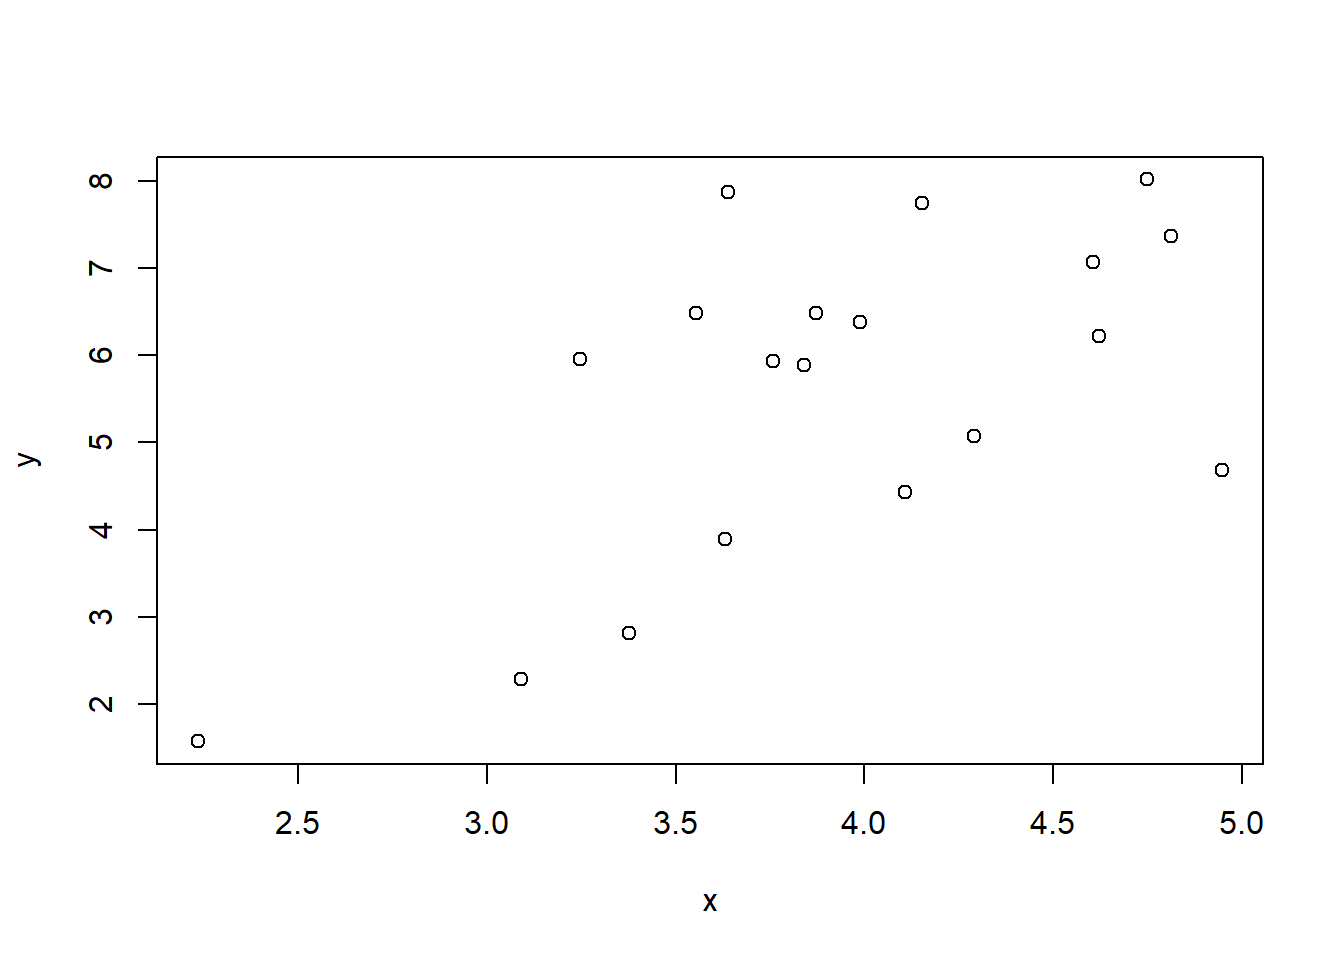
\includegraphics{bookdown-demo_files/figure-latex/diagram-pencar-1.pdf}
\caption{\label{fig:diagram-pencar}Diagram Pencar Penjualan Motor (y) sebagai Fungsi dari Pendapatan per Kapita (x)}
\end{figure}

Selanjutnya kita tambahkan sebuah garis lurus yang paling banyak ``mendekati'' titik-titik data pengamatan yang tersebar. Sebuah garis lurus yang kita tarik seperti pada Gambar 1.2 menunjukkan bahwa proporsionalitas ini memang ada tetapi tidak ketat. Garis lurus yang kita tambahkan tidak menyinggung seluruh data yang tersebar. Dengan kata lain data sampel tidak bisa seluruhnya tepat berada pada garis yang dibuat. Titik-titik pengamatan ada yang tepat digaris, ada juga yang di atas atau di bawah garis.

Ini menunjukkan adanya \textbf{variasi} pada penjualan motor yang tidak berhubungan dengan tingkat pendapatan. Atau terdapat faktor-faktor lain selain pendapatan yang juga mempengaruhi tingkat penjualan tetapi tidak tercakup di dalam model.

\begin{figure}
\centering
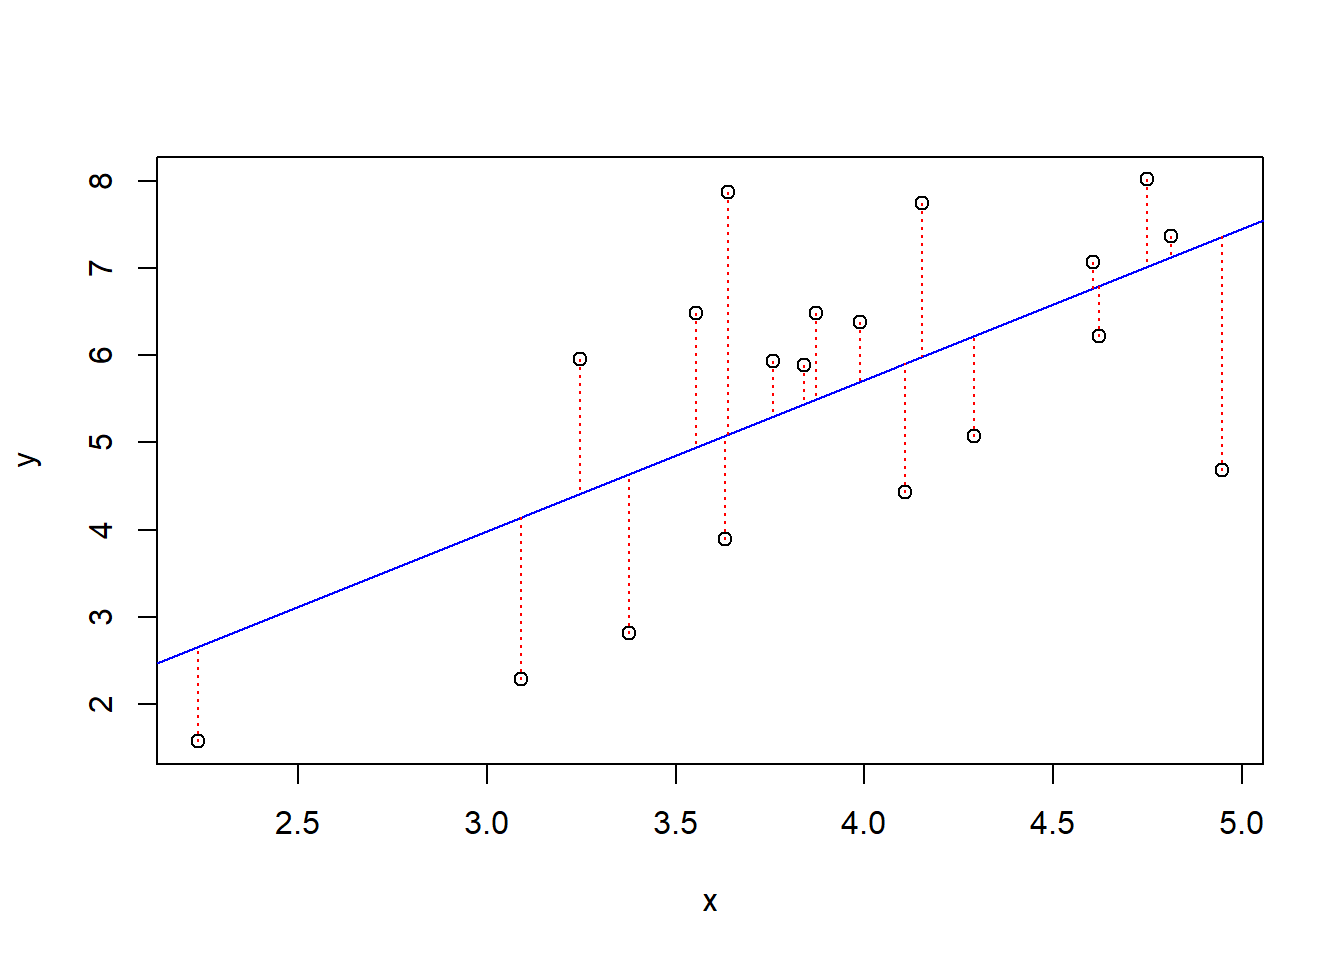
\includegraphics{bookdown-demo_files/figure-latex/garis-regresi-1.pdf}
\caption{\label{fig:garis-regresi}Garis Regresi Penjualan Motor (y) sebagai Fungsi dari Pendapatan per Kapita (x)}
\end{figure}

Jika kita ekspresikan ke dalam persamaan, garis regresi yang memodelkan hubungan antara \(y\) dan \(x\) dapat kita tuliskan sebagai:

\begin{equation} 
y_i=\beta_0 + \beta_1x_i
\label{eq:persamaan-noerror}
\end{equation}

Persamaan ini menyatakan bahwa \(y\) sebagai variabel respons adalah fungsi linier dari \(x\), variabel prediktor. \(\beta_0\) adalah intersep (\emph{intercept}) yang menunjukkan nilai dari \(y\) jika \(x\) sama dengan nol. \(\beta_1\) adalah koefisien kemiringan garis (\emph{slope}) yang menunjukkan berapa banyak \(y\) akan berubah jika \(x\) meningkat sebanyak satu unit.

Di dalam analisis regresi kita mencari nilai dugaan \(\hat \beta_0\) dan \(\hat \beta_1\) sehingga rata-rata jarak vertikal untuk setiap titik data pengamatan dengan nilai dugaannya secara kolektif paling
kecil (Gambar 1.3). Dengan kata lain kita ingin menarik garis regresi dalam bidang x−y sedekat mungkin dengan persebaran titik-titik data sampel yang telah
kita kumpulkan sehingga variasi yang tidak dapat dijelaskan oleh model menjadi minimum.

Salah satu cara untuk mendapatkan garis yang paling pas (\emph{line of best fit}) yang sangat populer adalah melalui suatu prosedur formal yang disebut \emph{metode kuadrat terkecil/ordinary least squares} (OLS). Sesuai namanya metode ini meminimalkan jumlah kuadrat kesalahan dari model.

\begin{figure}
\centering
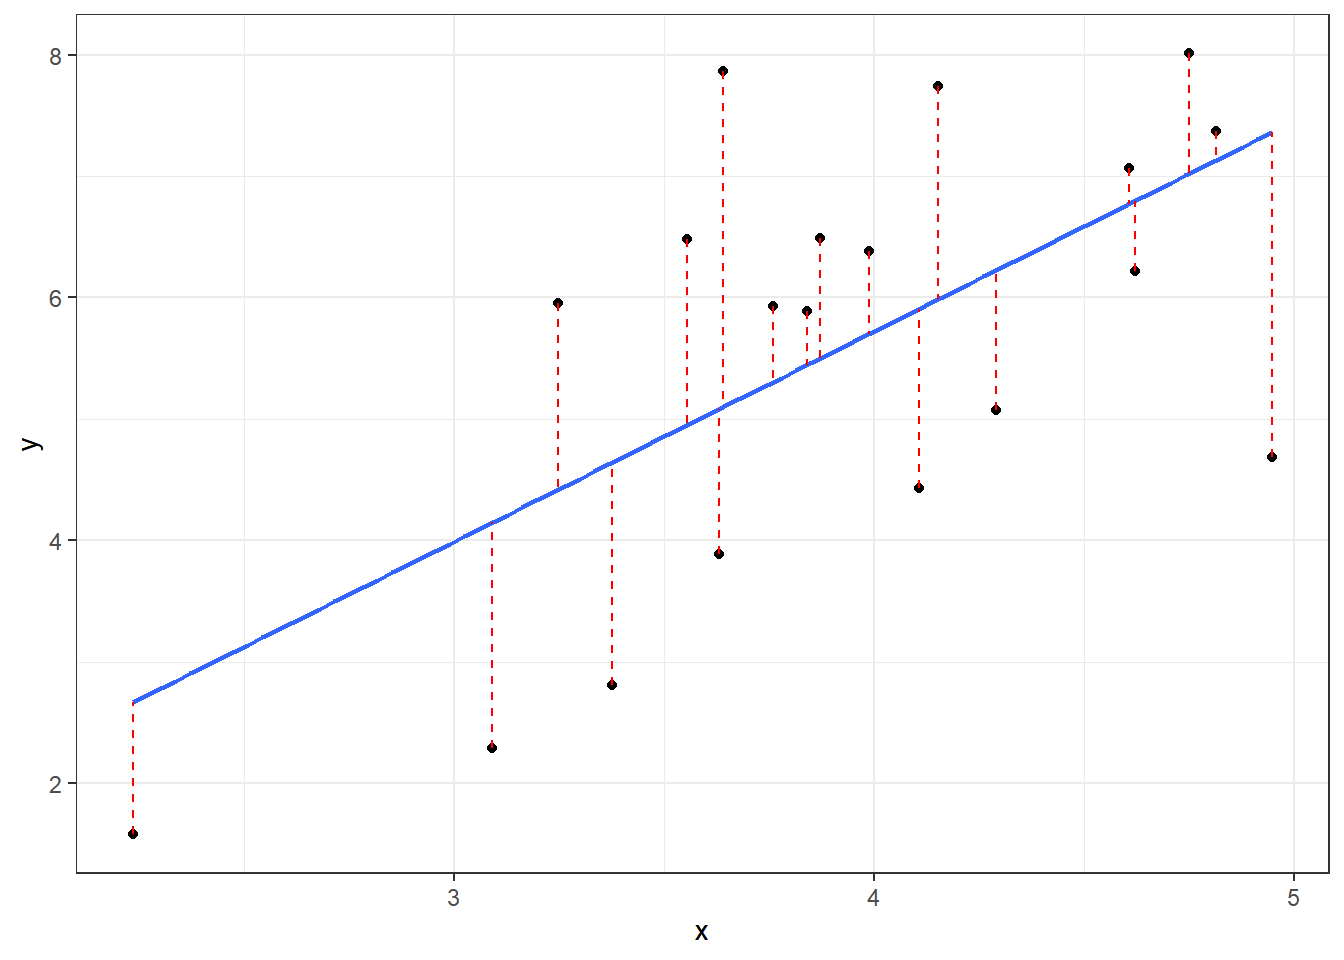
\includegraphics{bookdown-demo_files/figure-latex/metode-ols-1.pdf}
\caption{\label{fig:metode-ols}Mencari Garis Regresi dengan Metode Kuadrat Terkecil}
\end{figure}

Di dalam kasus penjualan motor, karena kita hanya menggunakan satu variabel prediktor dalam regresi sederhana, faktor lain selain pendapatan yang menyebabkan variasi pada penjualan motor kita masukkan sebagai faktor acak (\emph{random factor}). Faktor acak ini secara visual ditunjukkan oleh panjang garis vertikal (warna merah putus-putus) antara titik data pengamatan dengan garis regresi atau nilai dugaan variabel respons (garis biru).

Faktor acak ini menunjukkan adanya variasi pada penjualan yang
tidak dapat dijelaskan oleh model dan disimbolkan dengan \(\epsilon\).
Maka persamaan garis regresi dapat kita tuliskan lagi sebagai:

\begin{equation} 
y_i=\beta_0 + \beta_1x_i + \epsilon_i
\label{eq:persamaan-witherror}
\end{equation}

\(\epsilon_i\) dimasukkan ke dalam persamaan untuk mengakomodasi variasi dalam \(y\) yang tidak dapat dijelaskan oleh variabel \(x\). Faktor acak ini adalah istilah
statistik yang mewakili fluktuasi acak, kesalahan pengukuran, atau
dampak dari faktor-faktor diluar kendali peneliti \citep{faraway2016a} yang menyebabkan nilai dugaan tidak sama dengan nilai aktual (\emph{error} atau residu). Jadi
\(\epsilon\) ini mewakili ketidakmampuan model untuk menjelaskan variasi
yang terjadi pada variabel respons.

Setiap model pasti mengandung \emph{error}, karena hubungan statistik tidak
memiliki ketepatan seperti halnya fungsi matematika. Jadi ketika kita
mencoba menjelaskan variabel \(y\) dengan menggunakan variabel \(x\) ini,
kita menggunakan hubungan statistik: sebuah hubungan yang tidak eksak.

Bahkan, seandainya variabel-variabel lain ditambahkan ke dalam model,
tetap akan ada variasi di dalam \(y\) yang tidak dapat dijelaskan oleh
model. Variasi ini bisa karena bentuk fungsional yang tidak benar atau
bisa juga karena semata-mata faktor kejadian yang tidak dapat
diprediksi.

Sebuah model regresi linier yang sudah dikalibrasi paling pas dengan
data sampel (\emph{the best fit}), dapat digunakan untuk menjelaskan hubungan
atau membuat prediksi dengan mencermati perbedaan (arah) dan intensitas
perubahan (magnitud) dari variabel \(y\) pada nilai variabel \(x\) tertentu.

Analisis regresi menawarkan pendekatan yang masuk akal dengan mengenali
pola-pola hubungan antar variabel: arah dan besar perubahan pada
variabel respons dengan arah dan besar perubahan pada variabel prediktor
dari model yang valid.

Dengan demikian persamaan regresi yang memodelkan hubungan statistik
antar variabel terdiri dari dua komponen: komponen deterministik atau
sinyal yaitu \(\beta_0 + \beta_1\) dan komponen acak yaitu \(\epsilon\). Kombinasi kedua komponen ini menjadikan persamaan regresi sebagai model non-eksak, yaitu bergantung pada bentuk-bentuk penjelasan probabilistik. Kita hanya mengasumsikan bahwa di dalam cakupan variabel yang dianalisis, terdapat tendensi variabel respons \(y\) untuk bervariasi secara sistematis dengan
variabel prediktor \(x\).

Mayoritas analisis regresi yang baku menggunakan model regresi linier,
yaitu mengasumsikan bahwa variabel respons dapat dituliskan sebagai
kombinasi linier dari variabel-variabel prediktornya. Beberapa alasan
mengapa model linier ini paling umum dipakai adalah \citep{rawlings1998}: (1)
model linier mudah dipahami; (2) beberapa model nonlinier secara
instrinsik linier, sehingga bisa didekati dengan pendekatan linier.

Dalam banyak hal, jumlah variabel respons yang kita analisis bisa lebih dari satu atau \(p>1\), sehingga persamaan umum regresinya menjadi:

\begin{equation} 
y_i=\beta_0 + \beta_1x_{i1} + \beta_2x_{i2} + ... + \beta_px_{ip} + \epsilon_i
\label{eq:persamaan-multi}
\end{equation}

Model ini disebut sebagai model regresi linier berganda. Disebut
berganda karena melibatkan lebih dari satu variabel
prediktor. Contoh-contoh penerapannya:

\begin{enumerate}
\def\labelenumi{\arabic{enumi}.}
\tightlist
\item
  Seorang mahasiswa ingin menduga koefisien-koefisien dari sebuah
  model yang menghubungkan bobot tanaman vaskular-tanaman yang
  memiliki jaringan khusus yaitu xilem dan floem untuk mengangkut
  unsur hara, air dan mineral ke seluruh bagian tanaman-dengan
  kandungan unsur hara dalam tanah, jumlah air yang diterima dan
  jangka waktu tanaman terpapar sinar matahari.
\item
  Kerja fisik (mengangkat, memutar, mendorong benda berat) tetap tidak
  dapat dihindari walaupun kita sudah mampu membuat alat-alat untuk
  membantu pekerjaan. Kadang pekerjaan itu harus kita lakukan dalam
  kondisi yang tidak ergonomis. Cedera tulang punggung seringkali
  ditemui pada pekerja di sektor ini. Seorang manajer produksi mungkin
  tertarik untuk mengurangi masalah cedera tulang belakang ini dengan
  menginvestigasi hubungan kepadatan mineral tulang belakang dengan
  usia, berat dan tinggi badan, jenis kelamin dan gaya hidup pekerja.
\item
  Seorang analis ingin mengetahui tingkat kepuasan karyawan sebuah
  perusahaan terhadap pekerjaannya. Skor total kepuasan kerja karyawan
  dihitung dari penjumlahan skor-skor 20 pertanyaan dengan menggunakan
  5 poin skala likert. Sedangkan prediktornya digunakan variabel
  demografi meliputi usia, jenis kelamin dan pendidikan terakhir
  karyawan.
\item
  Di dalam teori konsumen, preferensi seorang konsumen terhadap suatu
  produk dipengaruhi oleh pengetahuan konsumen terhadap produk,
  emosi,\emph{word of mouth}, faktor-faktor personal dan lingkungan.
\end{enumerate}

\hypertarget{asumsi-asumsi-model-linier}{%
\section{Asumsi-Asumsi Model Linier}\label{asumsi-asumsi-model-linier}}

\emph{All models are wrong, but some are useful} \citep{box1979}. Seperti
halnya metodologi statistik yang lain, analisis regresi linier dapat
menjadi cara yang sangat efektif untuk memodelkan data sepanjang
asumsi-asumsinya terpenuhi. Jika asumsinya tidak terpenuhi, metode kuadrat
terkecil berpotensi memberikan hasil yang arahnya tidak tepat
(\emph{misleading}).

Setelah analisis regresi dilakukan, kita harus melakukan uji diagnostik:
memastikan apakah model memenuhi asumsi-asumsi model linier. Uji
diagnostik dapat dilakukan secara grafik maupun dengan uji formal.

Asumsi-asumsi regresi linier adalah:

\begin{enumerate}
\def\labelenumi{\arabic{enumi}.}
\tightlist
\item
  Linieritas data: hubungan antara prediktor \(x\) dengan respons \(y\)
  diasumsikan linier.
\item
  Normalitas residu. error/residu diasumsikan terdistribusi secara
  normal.
\item
  Homogenitas variansi residu: residu diasumsikan mempunyai variansi
  yang tetap (homoskedastisitas)
\item
  Independensi residu.
\end{enumerate}

Potensi-potensi tidak terpenuhinya asumsi model regresi adalah:

\begin{enumerate}
\def\labelenumi{\arabic{enumi}.}
\tightlist
\item
  Hubungan antara respons dengan prediktor tidak linier
\item
  Heteroskedastisitas: variansi residu tidak tetap.
\item
  Adanya nilai-nilai yang ``berpengaruh'' besar yang berasal dari (a)
  nilai pencilan (\emph{outlier}) yaitu nilai-nilai ekstrim pada variabel
  respons; (b) high-leverage points: nilai-nilai ekstrim pada variabel
  prediktor.
\end{enumerate}

Uji hipotesis, interval dan prediksi didasarkan atas kepercayaan bahwa asumsi-asumsi model regresi dipenuhi. Jadi penting sekali untuk melakukan pengecekan terhadap asumsi-asumsi ini. Jika asumsi-asumsi dipenuhi, berbagai bentuk inferensi seperti prediksi, kontrol, ekstraksi informasi, penemuan pengetahuan dan evaluasi risiko dapat dilakukan dengan kerangka argumen deduktif sesuai dengan model yang dibangun.

\hypertarget{uji-signifikansi}{%
\section{Uji Signifikansi}\label{uji-signifikansi}}

Salah satu fungsi dari regresi linier adalah untuk estimasi kondisi
populasi. Kita mengamati dan mengumpulkan data sampel, tetapi kita ingin
mengetahui apakah data sampel yang kita miliki juga menerangkan sesuatu
tentang populasi dimana data ini diambil. Dengan kata lain kita ingin
mengetahui apakah hasil dari analisis data sampel dapat digeneralisasi
ke populasi dengan uji signifikansi.

Uji signifikansi dapat dilakukan jika asumsi-asumsi model regresi telah
dipenuhi. Uji-uji signifikansi itu antara lain:

\begin{enumerate}
\def\labelenumi{\arabic{enumi}.}
\item
  Uji t: digunakan untuk mengetahui apakah koefisien-koefisien regresi
  secara statistik berbeda secara signifikan
  (\emph{statistically-significantly}) dari nol.
\item
  Uji F: jika uji t digunakan untuk menguji hanya satu koefisien, uji
  F digunakan untuk menguji lebih dari satu koefisien secara serempak.
\end{enumerate}

\hypertarget{langkah-langkah-melakukan-analisis-regresi}{%
\section{Langkah-langkah Melakukan Analisis Regresi}\label{langkah-langkah-melakukan-analisis-regresi}}

Berdasarkan uraian sebelumnya, secara umum langkah-langkah dalam melakukan analisis regresi adalah sebagai berikut:

\begin{enumerate}
\def\labelenumi{\arabic{enumi}.}
\tightlist
\item
  Menentukan variabel respons \(y\) yang akan kita pelajari atau buat
  modelnya.
\item
  Menentukan sejumlah variabel prediktor yang kita anggap berguna di
  dalam menjelaskan variabel respons.
\item
  Mengumpulkan data (sampel) yang dapat digunakan untuk menguji model.
\item
  Mengestimasi model.
\item
  Cek kecukupan model/uji diagnostik (jika hasilnya kurang memuaskan,
  kembali ke tahap 1).
\item
  Uji signifikansi dan inferensial.
\item
  Menulis hasil analisis.
\end{enumerate}

\hypertarget{penggunaan-komputer}{%
\section{Penggunaan Komputer}\label{penggunaan-komputer}}

Jika diperhatikan langkah-langkah untuk melakukan analisis regresi pada
1.3, membangun model regresi merupakan sebuah proses iteratif. Dimulai
dengan kajian teori yang berhubungan topik yang sedang diteliti dan
ketersediaan data untuk menentukan variabel respons dan variabel
eksplanatori untuk membangun model awal.

Salah satu pertimbangan penting di dalam memilih variabel prediktor
adalah apakah variabel tersebut dapat mengurangi variasi dalam variabel
respons. Pertimbangan lain adalah seberapa mudah, murah dan akurat data
variabel itu bisa diperoleh dibandingkan calon variabel prediktor yang
lain. Pemilihan ini harus cermat karena bagaimanapun model adalah sebuah
penyederhanaan dari realitas yang lebih kompleks, sehingga sebaiknya
beberapa prediktor saja dimasukkan ke dalam model.

Menampilkan data dalam grafik atau diagram pencar seringkali sangat
berguna untuk spesifikasi model awal. Setelah itu parameter-parameter
model diestimasi. Setelah itu kecukupan model dievaluasi yang meliputi
mencari kemungkinan terjadi kesalahan spesifikasi model, kemungkinan
tidak memasukkan variabel penting atau memasukkan variabel yang tidak
perlu, menemukan data pencilan (\emph{outlier}).

Kecukupan dan kecocokan model harus dicek karena menentukan apakah model
yang dibuat dapat dipakai atau tidak. Hasil dari cek kecukupan mungkin
mengindikasikan apakah model yang dibuat cukup masuk akal atau perlu
dimodifikasi. Di dalam uji kecukupan terutama yang perlu dicek adalah
residu sebagai realisasi dari kesalahan model \(\epsilon\).

Jika model tidak cukup memenuhi, maka perlu dilakukan tindakan perbaikan
dan pendugaan paramater diulang lagi. Proses ini mungkin perlu diulang
beberapa kali sampai diperoleh model yang memuaskan. Selanjutnya
dilakukan validasi untuk memastikan bahwa model dapat diterima di dalam
tahap akhir penerapannya.

Dengan demikian, analisis regresi seringkali melibatkan banyak
penghitungan, apalagi jika jumlah sampelnya besar dan variabel
prediktornya banyak. Untuk membantu mempercepat proses ini kita menggunakan program komputer.

Program komputer yang bagus adalah alat yang diperlukan dalam proses
membangun model. Tetapi program komputer saja belum cukup. Analisis
regresi memerlukan seni dan inteligensia dalam penggunaan komputer.
Analis harus belajar bagaimana menginterpretasikan output komputer dan
mengintegrasikan informasi yang didapat dengan model-model yang akan
dibuat selanjutnya.

Berbagai program statistik seperti SPSS, Stata, Minitab, Eviews, SAS,
JMP, R, dan lain-lain dapat melakukan penghitungan regresi secara cepat
dengan hasil yang kurang lebih sama. Di buku ini saya menggunakan
software R \citep{rcoreteam2021} untuk membuat grafik maupun penghitungan
regresinya.

\hypertarget{regresi-linier-sederhana}{%
\chapter{Regresi Linier Sederhana}\label{regresi-linier-sederhana}}

Bab ini akan membahas regresi linier sederhana. Istilah regresi sederhana tidak merujuk pada kenaifan penelitiannya tetapi merujuk pada model yang hanya terdiri dari satu variabel respons dan satu variabel prediktor.

Situasi ini sering terjadi pada penelitian sains. Misalnya seorang peneliti ingin memprediksi laju reaksi kimia karena perubahan temperatur, atau ingin mengetahui hubungan antara perubahan diet dengan tingkat kolesterol pada seseorang. Jika dapat diasumsikan bahwa variabel-variabel ini terhubung secara linier, kita dapat menggunakan regresi linier sederhana untuk mengkuantifikasi hubungan ini.

Analisis regresi digunakan ketika solusi eksak tidak tersedia, dalam arti kita tidak akan dapat menemukan nilai tunggal yang dapat mencakup secara lengkap hubungan antara variabel respons dengan prediktornya. Sehingga disini kita mencoba memprediksi setepat mungkin variabel respons atau memprediksi dengan kesalahan terkecil.

Untuk mencapai tujuan ini, kita menganalisis pola-pola variabilitas pada variabel respons dan mencoba melihat apakah variabilitas ini dapat diprediksi dari variabilitas prediktornya.

\hypertarget{model-regresi-linier-sederhana}{%
\section{Model Regresi Linier Sederhana}\label{model-regresi-linier-sederhana}}

Model regresi linier sederhana dapat dituliskan sebagai berikut:

\begin{equation} 
y_i=\beta_0 + \beta_1x_i+ \epsilon_i
\label{eq:persamaan-umum}
\end{equation}

Regresi sederhana mengindikasikan hanya ada satu variabel prediktor x untuk menduga variabel respons y. Linier disini diartikan modelnya linier pada parameternya dalam hal ini \(\beta_0\) dan \(\beta_1\). Jadi model \(y_i = \beta_0 + \beta_1{x_i}^2 + \epsilon_i\) adalah linier pada \(\beta_0\) dan \(\beta_1\), sementara model \(y_i = \beta_0 + e^{\beta_ix_i} + \epsilon_i\) tidak linier.

Misalkan kita memiliki pasangan-pasangan data sampel sebanyak n yang diambil secara acak dari populasi yang lebih besar \((x_1,y_1), (x_2,y_2), ⋯, (x_n,y_n)\). Tujuan dari analisis regresi linier adalah menemukan model terbaik yaitu menemukan nilai \(\beta_0\) and \(\beta_1\) yang menghasilkan garis paling cocok dengan titik-titik data yang kita punyai.

Dengan kata lain tujuan dari analisis regresi adalah mengestimasi koefisien regresi untuk variabel prediktor sehingga didapatkan nilai dugaan variabel respons sedekat mungkin nilainya dengan nilai pengamatan aktualnya.

Di dalam analisis regresi, model terbaik ditunjukkan oleh garis lurus yang menghubungkan rata-rata variabel prediktor dengan variabel respons sedemikian rupa sehingga jumlah kuadrat kesalahan (jarak vertikal antara titik-titik data pengamatan aktual \(y_i\) dengan nilai dugaannya \(\hat y_i\)) minimal.

Untuk memperoleh nilai dugaan \(\beta_0\) dan \(\beta_1\) yang paling cocok, kita menggunakan metode kuadrat terkecil (\emph{method of least squares}). Dengan pendekatan kuadrat terkecil, kita mencari nilai dugaan \(\beta_0\) dan \(\beta_1\) yang meminimalkan jumlah kuadrat residu/kesalahan (\(y_i-\hat y_i\)).

\hypertarget{kasus-1-penjualan-motor-dan-pertumbuhan-pendapatan-perkapita}{%
\subsection{Kasus 1: Penjualan Motor dan Pertumbuhan Pendapatan Perkapita}\label{kasus-1-penjualan-motor-dan-pertumbuhan-pendapatan-perkapita}}

Kita akan melanjutkan kasus hubungan antara penjualan motor dengan pendapatan pada Bab 1 sebelumnya sebagai ilustrasi regresi linier sederhana. Data dapat diunduh di \href{https://drive.google.com/file/d/1Aa6A0KkXXINoDkdNJSnYUY5Y0E1xnrOb/view?usp=sharing}{sini}. Langkah awal untuk melihat bagaimana hubungan antar variabel adalah membuat diagram pencar.

Plot sangat penting di dalam regresi. Pemeriksaan diagram pencar secara teliti harus mendahului penghitungan regresi. Diagram pencar dapat mengindikasikan apakah model regresi yang diinginkan mungkin masuk akal atau tidak. Kesepakatan dalam membuat diagram pencar, variabel \(x\) sebagai variabel penjelas diplot pada sumbu horisontal. Varibel \(y\) sebagai variabel respons diplot pada sumbu vertikal.

Untuk membuat diagram pencar, hal pertama yang harus dilakukan adalah memasukkan data ke dalam R, mengecek apakah data yang kita masukkan sudah betul dan memanggil \emph{package} yang relevan dengan model yang akan dibuat.

\begin{Shaded}
\begin{Highlighting}[]
\CommentTok{\# memanggil data yang disimpan dalam bentuk teks ke dalam R}
\NormalTok{PJMotor }\OtherTok{\textless{}{-}} \FunctionTok{read.delim}\NormalTok{(}\StringTok{"PJMotor.txt"}\NormalTok{) }
\NormalTok{PJMotor }\OtherTok{\textless{}{-}} \FunctionTok{as.data.frame}\NormalTok{(PJMotor)}
\end{Highlighting}
\end{Shaded}

\begin{Shaded}
\begin{Highlighting}[]
\CommentTok{\# untuk melihat beberapa baris data teratas}
\FunctionTok{head}\NormalTok{(PJMotor) }
\end{Highlighting}
\end{Shaded}

\begin{verbatim}
##   Tahun        y        x
## 1  2001 1.575822 2.235180
## 2  2002 2.287706 3.090636
## 3  2003 2.809896 3.376533
## 4  2004 3.887678 3.630909
## 5  2005 5.074186 4.289591
## 6  2006 4.428274 4.107514
\end{verbatim}

\begin{Shaded}
\begin{Highlighting}[]
\CommentTok{\# untuk melihat beberapa baris data terakhir}
\FunctionTok{tail}\NormalTok{(PJMotor) }
\end{Highlighting}
\end{Shaded}

\begin{verbatim}
##    Tahun        y        x
## 14  2014 7.867195 3.639072
## 15  2015 6.480155 3.555062
## 16  2016 5.931285 3.758837
## 17  2017 5.886103 3.841197
## 18  2018 6.383108 3.987825
## 19  2019 6.487460 3.871444
\end{verbatim}

Data yang kita masukkan kelihatan seperti yang diharapkan. Variabel penjualan dan pendapatan semua dibaca sebagai angka (\emph{numeric data type}). Selanjutnya kita akan lihat struktur dan ringkasan persebaran datanya.

\begin{Shaded}
\begin{Highlighting}[]
\CommentTok{\# melihat struktur data}
\FunctionTok{str}\NormalTok{(PJMotor)}
\end{Highlighting}
\end{Shaded}

\begin{verbatim}
## 'data.frame':    19 obs. of  3 variables:
##  $ Tahun: int  2001 2002 2003 2004 2005 2006 2007 2008 2009 2010 ...
##  $ y    : num  1.58 2.29 2.81 3.89 5.07 ...
##  $ x    : num  2.24 3.09 3.38 3.63 4.29 ...
\end{verbatim}

Hasil fungsi \texttt{str()} menunjukkan bahwa data ini adalah data \emph{time series} terdiri dari tiga kolom yaitu penjualan motor (y), pertumbuhan pendapatan per kapita (x) dan tahun selama 19 tahun dari 2001-2019.

\begin{Shaded}
\begin{Highlighting}[]
\CommentTok{\# melihat ringkasan data kecuali data tahun}
\FunctionTok{summary}\NormalTok{(}\FunctionTok{subset}\NormalTok{(PJMotor, }\AttributeTok{select =} \FunctionTok{c}\NormalTok{(y,x)))}
\end{Highlighting}
\end{Shaded}

\begin{verbatim}
##        y               x        
##  Min.   :1.576   Min.   :2.235  
##  1st Qu.:4.558   1st Qu.:3.593  
##  Median :5.952   Median :3.871  
##  Mean   :5.587   Mean   :3.922  
##  3rd Qu.:6.776   3rd Qu.:4.448  
##  Max.   :8.013   Max.   :4.946
\end{verbatim}

Selanjutnya kita cek normalitas data, korelasi dan diagram pencar antara pasangan data \(y\) dengan \(x\) seperti yang ditunjukkan pada Gambar 2.1.

\begin{Shaded}
\begin{Highlighting}[]
\FunctionTok{library}\NormalTok{ (GGally)}
\NormalTok{GGally}\SpecialCharTok{::}\FunctionTok{ggpairs}\NormalTok{(}\FunctionTok{subset}\NormalTok{(PJMotor, }\AttributeTok{select =} \FunctionTok{c}\NormalTok{(y,x)))}
\end{Highlighting}
\end{Shaded}

\begin{figure}[H]

{\centering 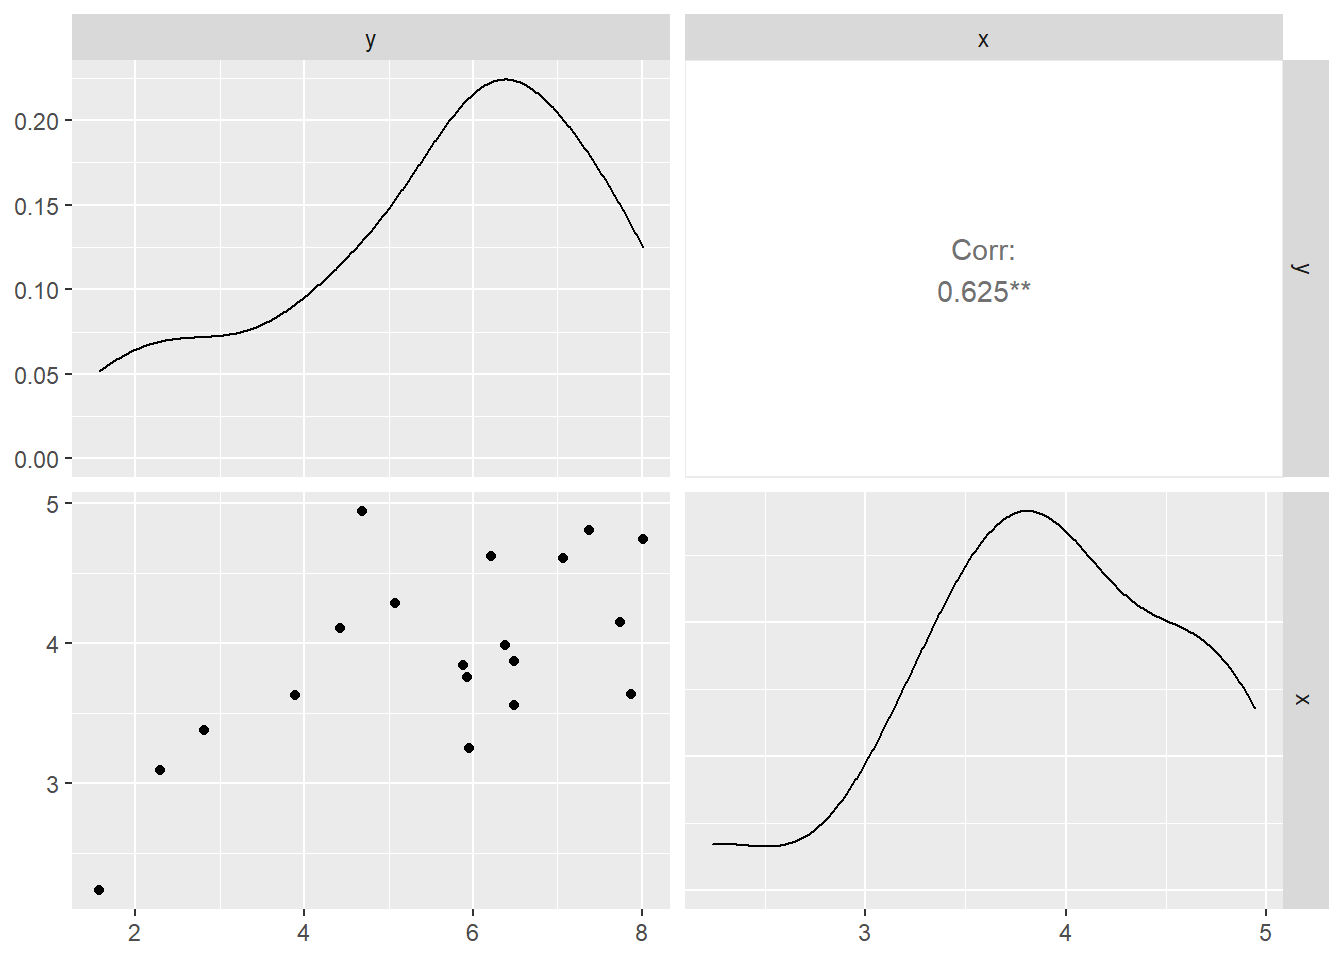
\includegraphics{bookdown-demo_files/figure-latex/plotpasangan-pjmotor-1} 

}

\caption{Plot Pasangan Data Penjualan dan Pendapatan}\label{fig:plotpasangan-pjmotor}
\end{figure}

Pada diagonal, kita melihat distribusi data \(y\) dan \(x\): data kedua variabel menceng ke kiri (\emph{skewed left}). Di atas diagonal ditunjukkan nilai korelasi antara \(y\) dan \(x\) yaitu sebesar=0.625. Koefisisen korelasi nilainya antara −1 (berkorelasi negatif sempurna) melalui 0 (tidak ada korelasi) sampai +1 (berkorelasi positif sempurna). Korelasi antara penjualan dan pendapatan disini positif cukup kuat dan signifikan. Grafik dibawah diagonal menunjukkan diagram pencar antara pasangan data \(y\) dengan \(x\) seperti yang sudah kita bahas sebelumnya di Bab 1.

Di dalam R model regresi linier sederhana dapat diperoleh dengan perintah \texttt{lm(y\textasciitilde{}x)}. Tanda \textasciitilde{} dapat diartikan \(y\) dijelaskan oleh \(x\) atau \(y\) fungsi dari \(x\). Fungsi ini mengestimasi koefisien regresi model linier dengan metode kuadrat terkecil (\emph{the least squares method}).

Semisal modelnya kita beri nama \textbf{model penjualan motor (mpm)}, yang memodelkan hubungan antara penjualan motor (\(y\)) dengan pertumbuhan pendapatan (\(x\)), maka model ini dapat diperoleh dengan perintah:

\begin{Shaded}
\begin{Highlighting}[]
\NormalTok{mpm }\OtherTok{\textless{}{-}} \FunctionTok{lm}\NormalTok{(y }\SpecialCharTok{\textasciitilde{}}\NormalTok{ x) }
\CommentTok{\# Perintah ini sama dengan y = β0 + β1x}
\CommentTok{\# Intersep secara default diestimasi. }
\CommentTok{\# Bandingkan dengan perintah untuk mendapatkan diagram pencar. }
\end{Highlighting}
\end{Shaded}

Kita kemudian menggunakan perintah \texttt{summary()} untuk menampilkan luarannya. Hasilnya adalah sebagai berikut:

\begin{Shaded}
\begin{Highlighting}[]
\CommentTok{\# perintah summary() untuk mengekstrak hasil regresi}
\FunctionTok{summary}\NormalTok{ (mpm) }
\end{Highlighting}
\end{Shaded}

\begin{verbatim}
## 
## Call:
## lm(formula = y ~ x)
## 
## Residuals:
##     Min      1Q  Median      3Q     Max 
## -2.6738 -1.1721  0.2916  0.9911  2.7707 
## 
## Coefficients:
##             Estimate Std. Error t value Pr(>|t|)   
## (Intercept)   -1.210      2.088  -0.579  0.56999   
## x              1.733      0.525   3.301  0.00422 **
## ---
## Signif. codes:  
## 0 '***' 0.001 '**' 0.01 '*' 0.05 '.' 0.1 ' ' 1
## 
## Residual standard error: 1.515 on 17 degrees of freedom
## Multiple R-squared:  0.3906, Adjusted R-squared:  0.3547 
## F-statistic: 10.89 on 1 and 17 DF,  p-value: 0.004224
\end{verbatim}

Persamaan regresinya dapat diringkas sebagai \(\hat penjualan=-1.21+1.73pendapatan\). Nilai dugaan intersep garis regresi \(\hat \beta_0\) = -1.210 (SE= 2.088), p-value = 0.57 (tidak signifikan). Nilai -1,21 menunjukkan dugaan penjualan sepeda motor (y dalam juta unit) jika pertumbuhan pendapatan per kapita sebesar 0 persen. Angka penjualan tidak mungkin negatif, paling rendah adalah 0. Jadi dalam kasus ini, nilai intersep dari model yang kita duga tidak mempunyai interpretasi yang berarti. Jadi intersep di dalam sebuah persamaan kadang-kadang mempunyai interpretasi yang berarti kadang juga tidak seperti dalam kasus kita ini.

Sedangkan nilai dugaan variabel prediktor pendapatan \(\hat \beta_1\) = 1.733 (SE = 0.525) dan p-valuenya (menguji hipotesis nol bahwa \(\beta_1\) = 0) kecil (signifikan), konsisten dengan bukti persebaran data yang cenderung linier. Jadi 1.733 adalah nilai kemiringan garis regresi yang menunjukkan untuk setiap perubahan pertumbuhan pendapatan per kapita sebesar 1\%, berkaitan dengan perubahan penjualan motor sebesar 1.73 juta unit. Jika terjadi kenaikan pertumbuhan pendapatan per kapita sebesar 1 persen, ini berkaitan dengan peningkatan penjualan motor sebanyak 1.73 juta unit.

Output lain yang penting dari perintah \texttt{summary()} adalah koefisisen determinasi (\(R^2\)) sebesar 0.39. Ini berarti pendapatan dapat menjelaskan sebesar 39\% variasi pada data penjualan motor. Dengan kata lain jika kita ingin menjelaskan mengapa penjualan motor naik turun, maka kita bisa melihat variasi pada pertumbuhan pendapatan. Tentu saja ada faktor lain yang menjelaskan fluktuasi penjualan motor. Tetapi karena model kita hanya memasukkan pendapatan sebagai variabel eksplanatori, maka cukup masuk akal jika model ini hanya menjelaskan sebanyak 39\%. Artinya terdapat 61\% variasi pada penjualan motor yang tidak bisa dijelaskan oleh pendapatan perkapita saja.

Selang kepercayaan batas atas dan batas bawah (95\% defaultnya) untuk nilai dugaan koefisien dapat diperoleh dengan perintah \texttt{confint()}.

\begin{Shaded}
\begin{Highlighting}[]
\CommentTok{\# perintah menampilkan selang kepercayaan}
\FunctionTok{confint}\NormalTok{(mpm)}
\end{Highlighting}
\end{Shaded}

\begin{verbatim}
##                 2.5 %   97.5 %
## (Intercept) -5.615467 3.196075
## x            0.625206 2.840601
\end{verbatim}

Terlihat bahwa selang kepercayaan untuk intersep meliputi angka 0 (tidak signifikan), sedangkan koefisien untuk pendapatan tidak meliputi 0 (signifikan).

\hypertarget{residu}{%
\subsubsection{Residu}\label{residu}}

Selisih antara nilai data aktual penjualan motor \(y_i\) dengan nilai dugaannya \(\hat y_i\) pada saat pendapatan \(x = x_i\) disebut residu. Nilai residu mencerminkan kegagalan garis regresi yang diestimasi untuk memodelkan pasangan data tersebut. Bagaimana nilai residu diperoleh secara detil?

\(\hat \beta_0\) dan \(\hat \beta_1\) adalah nilai-nilai koefisien garis regresi dengan menggunakan data sampel sebanyak 19 tahun \((x_1, y_1),(x_2, y_2), . . . , (x_{19}, y_{19})\). Untuk setiap pertumbuhan pendapatan per tahun sebesar \(x\), nilai dugaaan penjualan motornya adalah sebesar \(\hat y = \hat \beta_0 + \hat \beta_1x\). Untuk setiap pertumbuhan pendapatan sebesar \(x_i\), dimana \(i = 1, 2, . . . , 19\), nilai selisih antara \(y_i−\hat y_i = y_i − (\hat \beta_0 + \hat \beta_1x_i)\) disebut residu.

Nilai residu ini dapat diperoleh dengan menggunakan perintah \texttt{augment()} dari \emph{broom package}. Misalkan residu dari perintah \texttt{augment()} kita sebut sebagai uji.diagnostik (dibahas secara lebih lengkap di Bab 4):

\begin{Shaded}
\begin{Highlighting}[]
\CommentTok{\# menambahkan nilai{-}nilai dugaan dan residu}
\CommentTok{\# library perlu dipanggil jika belum dipanggil sebelumnya}
\CommentTok{\# library("broom") }
\NormalTok{uji.diagnostik }\OtherTok{\textless{}{-}} \FunctionTok{augment}\NormalTok{(mpm)}
\FunctionTok{head}\NormalTok{(uji.diagnostik)}
\end{Highlighting}
\end{Shaded}

\begin{verbatim}
## # A tibble: 6 x 8
##       y     x .fitted .resid   .hat .sigma .cooksd
##   <dbl> <dbl>   <dbl>  <dbl>  <dbl>  <dbl>   <dbl>
## 1  1.58  2.24    2.66  -1.09 0.394    1.52  0.277 
## 2  2.29  3.09    4.15  -1.86 0.136    1.48  0.136 
## 3  2.81  3.38    4.64  -1.83 0.0883   1.49  0.0776
## 4  3.89  3.63    5.08  -1.19 0.0628   1.53  0.0222
## 5  5.07  4.29    6.22  -1.15 0.0689   1.53  0.0228
## 6  4.43  4.11    5.91  -1.48 0.0568   1.51  0.0304
## # ... with 1 more variable: .std.resid <dbl>
\end{verbatim}

Kolom-kolom pada tabel diatas menunjukkan

\begin{verbatim}
x: pertumbuhan pendapatan per kapita
y: penjualan motor aktual
.fitted: nilai dugaan penjualan motor
.resid: nilai residu (penjualan motor aktual-nilai dugaan penjualan motor)
\end{verbatim}

Kode berikut memplot nilai residu (warna merah) yaitu selisih antara nilai pengamatan aktual dengan nilai dugaan. Setiap garis vertikal warna merah menunjukkan nilai residu antara data penjualan motor aktual dengan nilai dugaannya.

\begin{Shaded}
\begin{Highlighting}[]
\CommentTok{\# library tidak perlu dipanggil lagi jika sudah dipanggil sebelumnya}
\CommentTok{\# library(ggplot2) }
\CommentTok{\# library(ggpmisc)}
\NormalTok{rumus }\OtherTok{\textless{}{-}}\NormalTok{ y }\SpecialCharTok{\textasciitilde{}}\NormalTok{ x}
\FunctionTok{ggplot}\NormalTok{(uji.diagnostik, }\FunctionTok{aes}\NormalTok{(x, y)) }\SpecialCharTok{+}
  \FunctionTok{geom\_point}\NormalTok{() }\SpecialCharTok{+}
  \FunctionTok{stat\_smooth}\NormalTok{(}\AttributeTok{method =} \StringTok{"lm"}\NormalTok{, }\AttributeTok{se =} \ConstantTok{FALSE}\NormalTok{, }\AttributeTok{formula =}\NormalTok{ rumus, }\AttributeTok{size =} \FloatTok{0.8}\NormalTok{) }\SpecialCharTok{+}
  \FunctionTok{geom\_segment}\NormalTok{(}\FunctionTok{aes}\NormalTok{(}\AttributeTok{xend =}\NormalTok{ x, }\AttributeTok{yend =}\NormalTok{ .fitted), }\AttributeTok{color =} \StringTok{"red"}\NormalTok{, }\AttributeTok{size =} \FloatTok{0.4}\NormalTok{, }\AttributeTok{linetype =} \StringTok{"dashed"}\NormalTok{) }\SpecialCharTok{+} 
  \FunctionTok{theme\_bw}\NormalTok{()}\SpecialCharTok{+}
   \FunctionTok{stat\_poly\_eq}\NormalTok{(}\AttributeTok{formula =}\NormalTok{ rumus,}
                \AttributeTok{eq.with.lhs =} \StringTok{"italic(hat(y))\textasciitilde{}\textasciigrave{}=\textasciigrave{}\textasciitilde{}"}\NormalTok{,}
                \FunctionTok{aes}\NormalTok{(}\AttributeTok{label =} \FunctionTok{paste}\NormalTok{(..eq.label.., ..rr.label.., }\AttributeTok{sep =} \StringTok{"\textasciitilde{}\textasciitilde{}\textasciitilde{}"}\NormalTok{)), }
                \AttributeTok{parse =} \ConstantTok{TRUE}\NormalTok{) }
\end{Highlighting}
\end{Shaded}

\begin{figure}[H]

{\centering 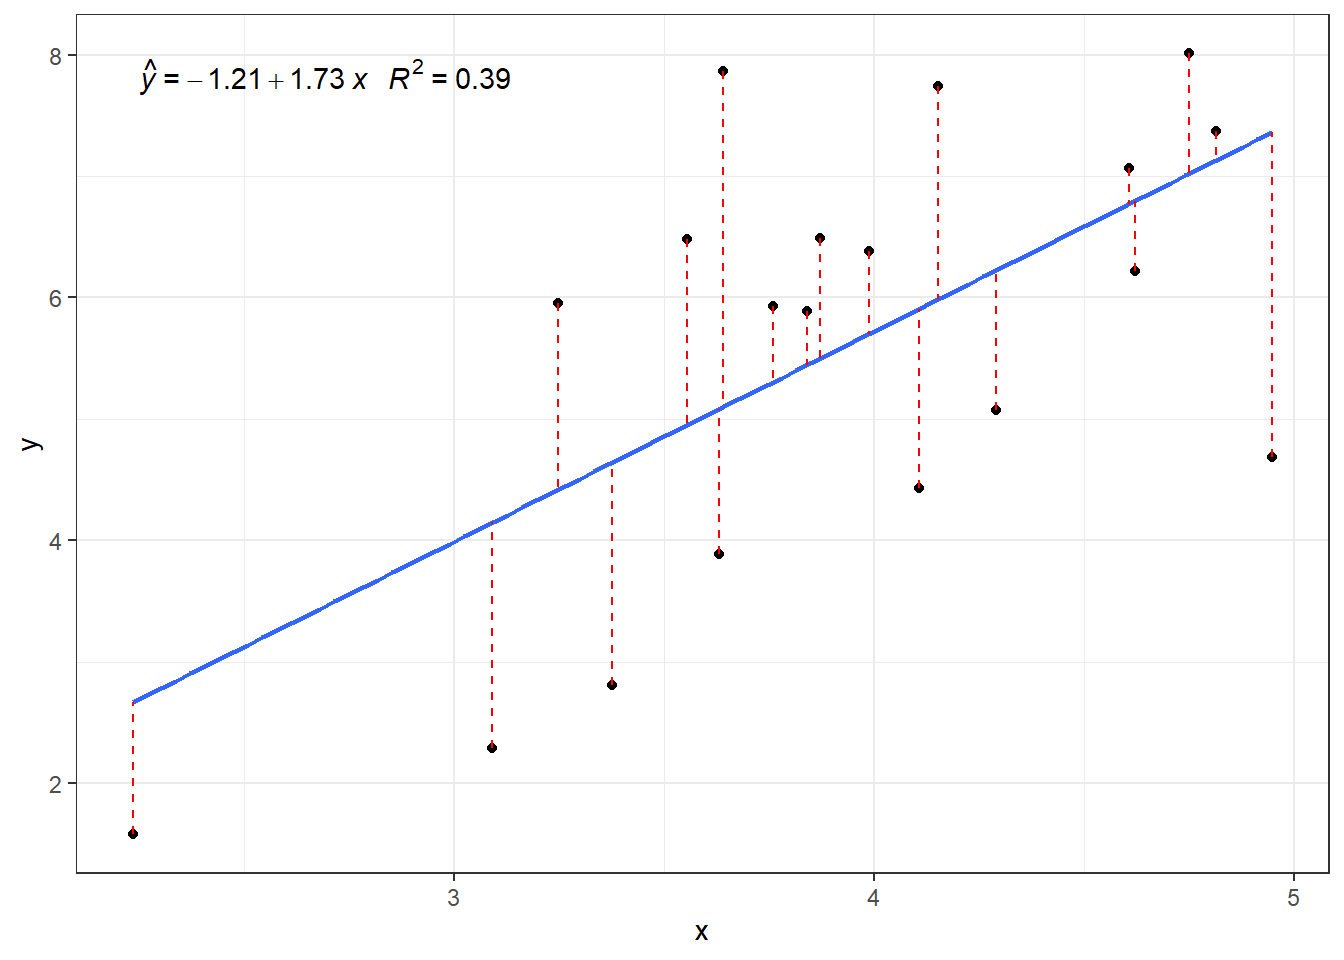
\includegraphics{bookdown-demo_files/figure-latex/plot-residu-mpm-1} 

}

\caption{Ilustrasi Geometrik dari OLS. Jarak antara Pengamatan dan Garis Regresi Sepanjang Sumbu y}\label{fig:plot-residu-mpm}
\end{figure}

\emph{work in progress}\ldots sedang dalam proses pengerjaan

\hypertarget{regresi-linier-berganda}{%
\chapter{Regresi Linier Berganda}\label{regresi-linier-berganda}}

Regresi linier berganda (\emph{multiple linear regression}) adalah pengembangan dari regresi linier sederhana. Dengan regresi linier berganda, kita dapat memasukkan lebih dari satu variabel penjelas ke dalam model. Hal ini dikarenakan di dalam praktik model yang kita pakai kemungkinan melibatkan lebih dari satu variabel prediktor.

Pengembangan ini bermanfaat jika dilihat dari dua sisi. Sisi pertama, penambahan variabel penjelas dapat memberikan penjelasan yang lebih lengkap tentang variabel respons, karena jarang suatu fenomena hanya disebabkan oleh hanya satu hal. Kedua, dampak dari variabel prediktor tertentu dibuat lebih terang, karena kemungkinan dampak distorsi dari variabel prediktor yang lain dihilangkan.

Pemahaman dasar-dasar dari regresi linier sederhana sangat penting untuk memahami regresi linier berganda yang lebih rumit. Dengan bantuan program komputer, proses estimasi dan interpretasi parameter mengikuti prinsip-prinsip yang sama. Begitu juga dengan uji signifikansi, koefisien determinasi (\(R^2\)) dan asumsi-asumsi pada regresi linier sederhana terus dibawa ke dalam regresi linier berganda.

Hal-hal yang harus diperhatikan karena berpotensi menjadi masalah dalam melakukan analisis regresi adalah isu-isu yang berhubungan (1) \emph{overfitting}, (2) heteroskedastisitas, (3) multikolinearitas. Teknik regresi berganda sangat luas cakupannya. Penguasaan teknik regresi berganda akan memberikan bekal yang sangat berharga untuk menganalisis berbagai jenis data kuantitatif.

\hypertarget{persamaan-umum}{%
\section{Persamaan Umum}\label{persamaan-umum}}

Secara umum, di dalam persamaan regresi berganda variabel respons dipandang sebagai fungsi linier dari \emph{lebih dari satu} variabel prediktor \(1>p\).

\begin{equation} 
y_i=\beta_0 + \beta_1x_{i1} + \beta_2x_{i2} + ... + \beta_px_{ip} + \epsilon_i
\label{eq:persamaan-ganda}
\end{equation}

Untuk model dengan dua variabel prediktor saja, persamaannya dapat dituliskan sebagai:

\begin{equation} 
y_i=\beta_0 + \beta_1x_{i1} + \beta_2x_{i2} + \epsilon_i
\label{eq:persamaan-2var}
\end{equation}

yang menunjukkan bahwa y ditentukan oleh \(x_1\) dan \(x_2\), ditambah faktor kesalahan. Untuk mengestimasi nilai-nilai parameter, kita gunakan prinsip kuadrat kesalahan terkecil (\emph{the least squares principle}), dengan meminimalkan jumlah kuadrat kesalahan prediksi (SSE):

\begin{equation}
SSE = \Sigma(y - \hat y)^2
\label{eq:persamaan-sse}
\end{equation}

Koefisien-koefisien yang diperoleh yaitu (\(\beta_0, \beta_1, \beta_2\)) menghasilkan kesalahan prediksi paling kecil dibandingkan kombinasi-kombinasi koefisien yang lain.
Tetapi disini kita tidak dapat lagi menampilkan diagram pencar pada bidang dua dimensi. Kita harus menampilkan perpencaran datanya pada bidang tiga dimensi. Lokasi dari garis pada bidang tiga dimensi ini ditentukan oleh besaran nilai-nilai (\(\beta_0, \beta_1, \beta_2\)). Jika variabel penjelasnya lebih dari tiga, perpencaran datanya sangat sulit untuk dibayangkan atau digambarkan.

sedang dalam proses pengerjaan (\emph{work in progress\ldots{}})

\hypertarget{uji-diagnostik-dan-tindakan-perbaikan}{%
\chapter{Uji Diagnostik dan Tindakan Perbaikan}\label{uji-diagnostik-dan-tindakan-perbaikan}}

Di dalam analisis regresi, kriteria jumlah kuadrat terkecil (OLS) tidak akan memberikan hasil yang memuaskan kecuali asumsi-asumsinya dipenuhi. Sampai saat ini kita belum melakukan uji asumsi-asumsi OLS. Uji diagnostik digunakan untuk melihat apakah asumsi-asumsi model dipenuhi atau terjadi pelanggaran pada asumsi-asumsi tersebut. Uji diagnostik biasanya menggunakan nilai residu/error.

Di bab ini kita akan menggunakan alat-alat yang dapat digunakan untuk mengidentifikasi dan mengatasi permasalahan-permasalahan yang biasa ditemui dalam penerapan metode kuadrat terkecil. Kita akan menggunakan baik cara grafik maupun rumus-rumus di dalam uji diagnostik ini.

\hypertarget{uji-asumsi-dengan-plotting-nilai-residu}{%
\section{Uji Asumsi dengan Plotting Nilai Residu}\label{uji-asumsi-dengan-plotting-nilai-residu}}

Hanya dengan melihat beberapa plot nilai residu bukti-bukti pemenuhan/pelanggaran asumsi OLS bisa kita dapatkan. Hal ini menjadi keunggulan uji diagnostik menggunakan grafik yaitu fleksibilitas. Hasil plot dapat menunjukkan bukti-bukti pelanggaran asumsi-asumsi serta tidak memerlukan spesifikasi pasti mengenai bentuk pelanggarannya. Fleksibilitas ini menjadi keunggulan sekaligus menjadi kelemahannya. Cara ini bersifat subjektif, sehingga orang berbeda bisa mempunyai pandangan yang berbeda pula mengenai validitas asumsi-asumsinya. Selain itu plot hanya bisa memberikan ``pandangan'' dua dimensi dari regresi berganda.

Beberapa plot untuk menguji asumsi OLS:

\begin{enumerate}
\def\labelenumi{\arabic{enumi}.}
\tightlist
\item
  Plot residu dengan nilai dugaan.
\item
  Plot residu dengan masing-masing prediktor.
\item
  Plot residu dengan waktu untuk data yang mengandung struktur waktu.
\item
  Plot normal residu.
\end{enumerate}

\hypertarget{plot-residu-dengan-nilai-dugaan.}{%
\subsection{Plot residu dengan nilai dugaan.}\label{plot-residu-dengan-nilai-dugaan.}}

\hypertarget{plot-residu-dengan-masing-masing-prediktor.}{%
\subsection{Plot residu dengan masing-masing prediktor.}\label{plot-residu-dengan-masing-masing-prediktor.}}

\hypertarget{plot-residu-dengan-waktu-untuk-data-yang-mengandung-struktur-waktu.}{%
\subsection{Plot residu dengan waktu untuk data yang mengandung struktur waktu.}\label{plot-residu-dengan-waktu-untuk-data-yang-mengandung-struktur-waktu.}}

\hypertarget{plot-normal-residu.}{%
\subsection{Plot normal residu.}\label{plot-normal-residu.}}

\hypertarget{uji-asumsi-dengan-tes-statistik}{%
\section{Uji Asumsi dengan Tes Statistik}\label{uji-asumsi-dengan-tes-statistik}}

sedang dalam proses pengerjaan (\emph{work in progress\ldots{}})

\hypertarget{model-regresi-linier-lanjutan}{%
\chapter{Model Regresi Linier Lanjutan}\label{model-regresi-linier-lanjutan}}

Ketika terjadi perubahan kuantitas sebuah variabel yang ada di dalam sebuah sistem, kita biasanya ingin tahu dampak dari perubahan itu terhadap kuantitas variabel-variabel lain yang ada di sistem tersebut. Hubungan perubahan ini mungkin cukup dimodelkan dengan hubungan fungsional sederhana. Bisa jadi juga hubungan perubahan ini lebih kompleks sehingga hubungan fungsional sederhana harus dikembangkan agar kita dapat menganalisisnya.
Persamaan umum model regresi dengan variabel respons \(y\) dan prediktor x sebanyak \(p\): \(x_1, x_2, ... , x_p\) adalah:

\begin{equation}
y = \beta_0 + \beta_1x_1 + ... + \beta_px_p + \epsilon
\label{eq:persamaan-lanjutan}
\end{equation}

dimana \(\epsilon\) terdistribusi secara normal. Persamaan di atas dapat dikembangkan berdasarkan tiga bagian penyusunnya. Bagian pertama adalah variabel responsnya \(y\), kedua adalah bagian residunya \(\epsilon\), dan ketiga adalah variabel prediktornya \(x\):

\begin{enumerate}
\def\labelenumi{\arabic{enumi}.}
\item
  \emph{Generalized Linear Models (GLM)}: Model linier standard tidak dapat mengakomodasi variabel respons \(y\) yang tidak normal seperti data dalam bentuk proporsi, persentase, binari, kategori dan \emph{count}. Di dalam kasus variabel respons yang kita hadapi seperti ini kita gunakan \emph{generalized linear model}.
\item
  \emph{Mixed Effect Model}: Model ini kita gunakan jika data kita tersusun secara hierarkis atau berkelompok. Misal untuk data pengamatan berulang, panel data, longitudinal dan data berjenjang yang mengakibatkan suatu struktur korelasi pada komponen errornya \(\epsilon\).
\item
  Model Regresi Nonparametrik (\emph{Nonparametric Regression Model}): Pada model linier, variabel prediktor \(x\) dikombinasikan secara linier untuk memodelkan dampaknya pada variabel respons. Akan tetapi kadang kala, linieritas ini tidak cukup menangkap struktur data sehingga diperlukan fleksibilitas lebih. Metode-metode yang dapat mengakomodasi ini misalnya \emph{additive model, trees and neural networks} memungkinkan pemodelan yang lebih fleksibel pada respons yang mengkombinasikan prediktor secara \emph{nonparametrik}.
\end{enumerate}

\hypertarget{generalized-linear-models-glm}{%
\section{\texorpdfstring{\emph{Generalized Linear Models (GLM)}}{Generalized Linear Models (GLM)}}\label{generalized-linear-models-glm}}

\hypertarget{mixed-effect-model}{%
\section{\texorpdfstring{\emph{Mixed Effect Model}}{Mixed Effect Model}}\label{mixed-effect-model}}

\hypertarget{model-regresi-nonparametrik}{%
\section{Model Regresi Nonparametrik}\label{model-regresi-nonparametrik}}

sedang dalam proses pengerjaan (\emph{work in progress\ldots{}})

  \bibliography{book.bib,packages.bib}

\end{document}
